\documentclass[a4paper,11pt]{report}

% We need more TeX registers
\usepackage{etex}
\usepackage[utf8]{inputenc}

\usepackage[a4paper, asymmetric, right=2.5cm, left=3.0cm, top=2.5cm, bottom=2.0cm]{geometry}

\usepackage[german, english]{babel}
\usepackage[left]{eurosym}
\usepackage{tabularx}
\newcolumntype{v}[1]{%
  >{\raggedright\hspace{Opt}}p{#1}%
}
\usepackage{slashbox}

\usepackage{tikz}
\usetikzlibrary{arrows}
\usetikzlibrary{shapes}
\usetikzlibrary{plotmarks}
\usetikzlibrary{decorations}
\usetikzlibrary{backgrounds,positioning}
\usepackage{amsmath}
\usepackage{amsfonts}
\usepackage{amssymb}
\usepackage{makeidx}
%\usepackage{multind}
\usepackage{tocbibind}
\usepackage{nicefrac}
\usepackage{thumbpdf}


\usepackage[draft=false, plainpages=false,
						colorlinks=true, linkcolor=blue, citecolor=blue, urlcolor=red,
						bookmarks, bookmarksopen, bookmarksopenlevel=1, bookmarksnumbered=true,breaklinks=true,
						pdftitle={The GrGen User Manual},
						pdfauthor={Jakob Blomer, Rubino Geiss, Edgar Jakumeit},
						pdfkeywords={
						graph, graph transformation, graph rewriting, tool, spo, manual, grgen, graph rewrite generator,
						University of Karlsruhe, IPD Goos},
						pdfpagelabels
						]{hyperref}

\usepackage[all]{xy}
\usepackage{xcolor}
\definecolor{light}{gray}{0.8}
\definecolor{tuerkis}{cmyk}{0.5,0.15,0,0.3}
\usepackage{picins} %wrapfig and floatflt suck deeply
\usepackage{graphicx}
\usepackage{calc}

%\usepackage{listings}
%\lstset{language=C, numbers=left, numberstyle=\tiny, stepnumber=5}

\providecommand{\O}[1]{\ensuremath{\mathcal{O}\left( #1 \right)}}

\providecommand{\N}{\ensuremath{\mathbb{N}}}
\providecommand{\Z}{\ensuremath{\mathbb{Z}}}
\renewcommand{\P}{\ensuremath{\mathbb{P}}}
\providecommand{\F}{\ensuremath{\mathbb{F}}}
\providecommand{\Q}{\ensuremath{\mathbb{Q}}}
\providecommand{\R}{\ensuremath{\mathbb{R}}}
\providecommand{\C}{\ensuremath{\mathbb{C}}}

\providecommand{\abs}[1]{\left\lvert #1 \right\rvert}
\providecommand{\norm}[1]{\left\lVert #1 \right\rVert}
\providecommand{\floor}[1]{\left\lfloor #1 \right\rfloor}
\providecommand{\svert}{\; \vert \;}

\DeclareMathOperator{\Abb}{Abb}   % Abbildungsmenge
\DeclareMathOperator{\Sym}{Sym}   % Bijektionenmenge
\DeclareMathOperator{\Hom}{Hom}   % Homomorphismenmenge
\DeclareMathOperator{\End}{End}   % Endomorphismenmenge
\DeclareMathOperator{\Aut}{Aut}   % Automorphismenmenge
\DeclareMathOperator{\deF}{def}
\DeclareMathOperator{\ran}{ran}
\DeclareMathOperator{\lhs}{lhs}
\DeclareMathOperator{\rhs}{rhs}

\providecommand{\id}{\ensuremath{\textsf{id}}}  % identische Abbildung
\DeclareMathOperator{\Kern}{Kern}     % Kern
\DeclareMathOperator{\Bild}{Bild}     % Bild

\providecommand{\Bin}[2]{\ensuremath{\operatorname{Bin} \left( #1 , #2 \right)}}
\providecommand{\Hyp}[2]{\ensuremath{\operatorname{Hyp} \left( #1 , #2 \right)}}

\providecommand{\PeroW}[2]{\ensuremath{\text{Per}^{#1}_{#2}\text{(oW)}}}
\providecommand{\PermW}[2]{\ensuremath{\text{Per}^{#1}_{#2}\text{(mW)}}}
\providecommand{\KomoW}[2]{\ensuremath{\text{Kom}^{#1}_{#2}\text{(oW)}}}
\providecommand{\KommW}[2]{\ensuremath{\text{Kom}^{#1}_{#2}\text{(mW)}}}

\makeatletter
\def\Relbar{\mathrel{\smash=}}
\def\Leftarrowfill@{\arrowfill@\Leftarrow\Relbar\Relbar}
\def\Rightarrowfill@{\arrowfill@\Relbar\Relbar\Rightarrow}
\newcommand{\xRightarrow}[2][]{\ext@arrow 0359\Rightarrowfill@{#1}{#2}}
\newcommand{\xLeftarrow}[2][]{\ext@arrow 3095\Leftarrowfill@{#1}{#2}}
\makeatother

\usepackage{rail}
\railalias{lbrace}{\{}
\railalias{rbrace}{\}}
\railalias{underscore}{\_}
\railalias{dollar}{\$}
\railalias{percent}{\%}
\railalias{ampersand}{<>}
\railalias{backslash}{\char"5C}
\railalias{tilde}{$\sim$}
\railalias{ampersand}{\&}
\railalias{doubleampersand}{\&\&}
\railalias{etc}{$\cdots$}
\railalias{xorhat}{$\wedge$}

\railalias{analyzegraph}{analyze\_graph}
\railalias{gensearchplan}{gen\_searchplan}
\railalias{setmaxmatches}{set\_max\_matches}
\railalias{dumpsourcecode}{dump\_sourcecode}

\railterm{lbrace,rbrace,dollar,percent,ampersand,backslash,underscore,tilde,ampersand,analyzegraph,gensearchplan,setmaxmatches,dumpsourcecode,doubleampersand,xorhat}

\usepackage[final]{listings}

\usepackage{soul}
\usepackage{titlesec}
\usepackage{titletoc}
\usepackage{fancyhdr}

% sectionreformatting
% tableofcontents level == 3 (subsubsection)
\setcounter{tocdepth}{3}
\setcounter{secnumdepth}{3}

% Headings
\pagestyle{myheadings}

\renewcommand{\chaptermark}[1]{\markboth{\it #1}{}}
\renewcommand{\sectionmark}[1]{\markright{\thesection \; \it #1}}
\lhead[\fancyplain{}{\thepage}]%
      {\fancyplain{}{\rightmark}}
\rhead[\fancyplain{}{\leftmark}]%
  {\fancyplain{}{\thepage}}
\renewcommand{\headrulewidth}{0pt}

\capsdef{////}{\upshape}{0.125em}{0.4583em}{0.5833em}
\newcommand{\versal}[1]{\MakeUppercase{\caps{#1}}}

% Other desccription labels, not that ugly bold font
% And put the description on a line of its own
\renewcommand\descriptionlabel[1]{%
  \hspace\labelsep {% local changes only
    \advance\linewidth\leftmargin
    \advance\linewidth-\labelsep
    \makebox[\linewidth][l]{\it #1}}}

% Other TOC headings for chapters \contentslabel{2.3em}}
%\titlecontents{chapter}[0em]{\sf\vspace*{2ex}}{Kapitel
%          \thecontentslabel{} --- }
%          {}{\hfill\contentspage\vspace*{1ex}}

\titlecontents{part}[0em]{\sf\large\vspace*{2ex}}{\contentslabel{2.3em}}
              {}{\hfill\contentspage\vspace*{1ex}}

\titlecontents{chapter}[0em]{\sf\vspace*{2ex}}{\contentslabel{2.3em}}
              {}{\hfill\contentspage\vspace*{1ex}}

%\titlecontents{chapter}[1.5em]{\sf}{2.3em}{1pc}{}{}{}
\dottedcontents{section}[3.8em]{}{2.3em}{1pc}

% Other formatting of chapter and section headings
\newcommand*\chaptitle[1]{\Large\filleft\versal{#1}}


\titleformat{\part}[block]
    {\LARGE\sf}
  {\versal{TEIL}\hspace*{2ex}\thepart}
  {4ex}{\Huge\newline\newline\centering}
\titleformat{\chapter}[display]
  {\large\sf}
  {\filright\versal{\chaptertitlename}\hspace*{2ex}\thechapter}
  {4ex}{\chaptitle}
\titleformat{\section}
  {\large\sf}{\thesection}
  {1em}{}
\titleformat{\subsection}
  {\sf}{\thesubsection}
  {1em}{}
\titleformat{\subsubsection}
  {\sf}{\thesubsubsection}
  {1em}{}
\titleformat{\paragraph}
  {\sf}{\theparagraph}{0em}{}
\titlespacing*{\paragraph}{0cm}{2.75ex plus 1ex minus .2ex}{.5em}

\makeatletter
\renewcommand*{\tableofcontents}{%
  \begingroup
    \@restonecolfalse
    \expandafter\chapter\expandafter*\expandafter{\contentsname}%
    \@mkboth{\contentsname}{\contentsname}%
    \@starttoc{toc}%
  \endgroup
} \makeatother



\selectlanguage{english}
\lstdefinelanguage{grgenmodel}
  {morekeywords={model, class, edge, node, connect, extends},
   sensitive=true,
   morecomment=[l]{\#},
  }
\lstdefinelanguage{grgenactions}
  {morekeywords={actions, using, rule, pattern, replace, negative},
   sensitive=true,
   morecomment=[l]{\#},
  }
\lstdefinelanguage{grshell}
  {morekeywords={},
   sensitive=true,
   morecomment=[l]{\#},
  }
\lstset{numbers=left, numberstyle=\tiny, stepnumber=1, firstnumber=auto, frame=single}
\providecommand{\GrG}{{\scshape GrGen}}
\newcommand{\lined}{\hfill \hrule\hfill\vspace{1mm} \\}

\title{\GrG\ User Manual \\ Graph Rewrite System}
\author{Jakob Blomer \\ \\ Institut für Programmstrukturen und Datenorganisation\\
Fakultät für Informatik\\
Universität Karlsruhe (TH)}

\begin{document}

\maketitle

\tableofcontents

\chapter{System Overview}

\GrG\ is a generative programming system for graph rewriting. \GrG\ is mainly designed for \emph{typed graphs}.  That means, graphs are not only nodes and edges, but labeled (\emph{attributed typed}) directed multigraphs. The type system is specified as class hierarchy, like a classes in object oriented languages. Type systems for specific sets of graphs can be specified by user supplied graph meta models. Such a graph model describes a set of well-formed graphs, i.e.\ allowed node and edge types, their attributes and specific connection assertions. We'll build a graph model for a turing machine in section \ref{anexample}.

How does graph rewriting work? \GrG\ implements an SPO-based approach. Given a host graph $H$, each \emph{rewriting rule} $p: L \longrightarrow R$ consists of a pattern $L$ and a transformation specification $R$ in form of a adopted pattern graph. The process of rewriting searches a match $H_L \unlhd H$ (i.e.\ a graph homomorphism from $L$ to a subgraph of $H$) and rewrites $H_L$ to $R$. Nodes or edges added to $R$ (in compare to $L$) will be added $H_L$ and nodes or edges deleted in $R$ will be deleted in $H_L$. The homomorphism may not be unique.

We'll have a look at a small example. First we use a special case to construct our host graph: an empty pattern does always produce exactly one match (independently of the host graph). So starting with an empty host graph $H$ we construct an apple using
\[ p:  \begin{array}[c]{c} \includegraphics[width=3cm]{fig/empty} \end{array} \begin{array}[c]{c} \longrightarrow \end{array} \begin{array}[c]{c} \includegraphics[width=3cm]{fig/apple} \end{array} \]
applied to $H$. We'll get the apple as new host graph $H'$. Now we want to rewrite our apple with stem to an apple with a leaflet. We use
\[ p':  \begin{array}[c]{c} \includegraphics[height=1.25cm]{fig/stiel} \end{array} \begin{array}[c]{c} \longrightarrow \end{array} \begin{array}[c]{c} \includegraphics[height=1.25cm]{fig/blatt} \end{array}, \]
apply $p'$ to $H'$ and get the new host graph $H''$, something like this:
\[ \includegraphics[width=3cm]{fig/wrongapple} \]
What happened? \GrG\ has randomly choosen a match, and $e3$ matches as well as $e1$. A correct solution could make use of edge type information. And this time we'll keep even the stem. So let $H''$ now be
\[ \includegraphics[width=3cm]{fig/typedapple} \]
and
\[ p'':  \begin{array}[c]{c} \includegraphics[height=1.25cm]{fig/typedstiel} \end{array} \begin{array}[c]{c} \longrightarrow \end{array} \begin{array}[c]{c} \includegraphics[height=1.25cm]{fig/typedblatt} \end{array}. \]
If we apply $p''$ to $H''$ this leads to
\[ \includegraphics[width=3cm]{fig/rewrittenapple} \]
\emph{Note:} If we had applied $(p')*$ to $H'$ (execute $p'$ consecutively until no match is found) this would not have terminated, because each rewrite had produced one new canditate (one deleted, two added) for matching.    

\section{Components}
Figure \ref{figsys} gives an overview of the \GrG\ system components, whereas table \ref{dirstruc} shows the \GrG\ directory structure.
\begin{figure}[htbp]
  \centering
  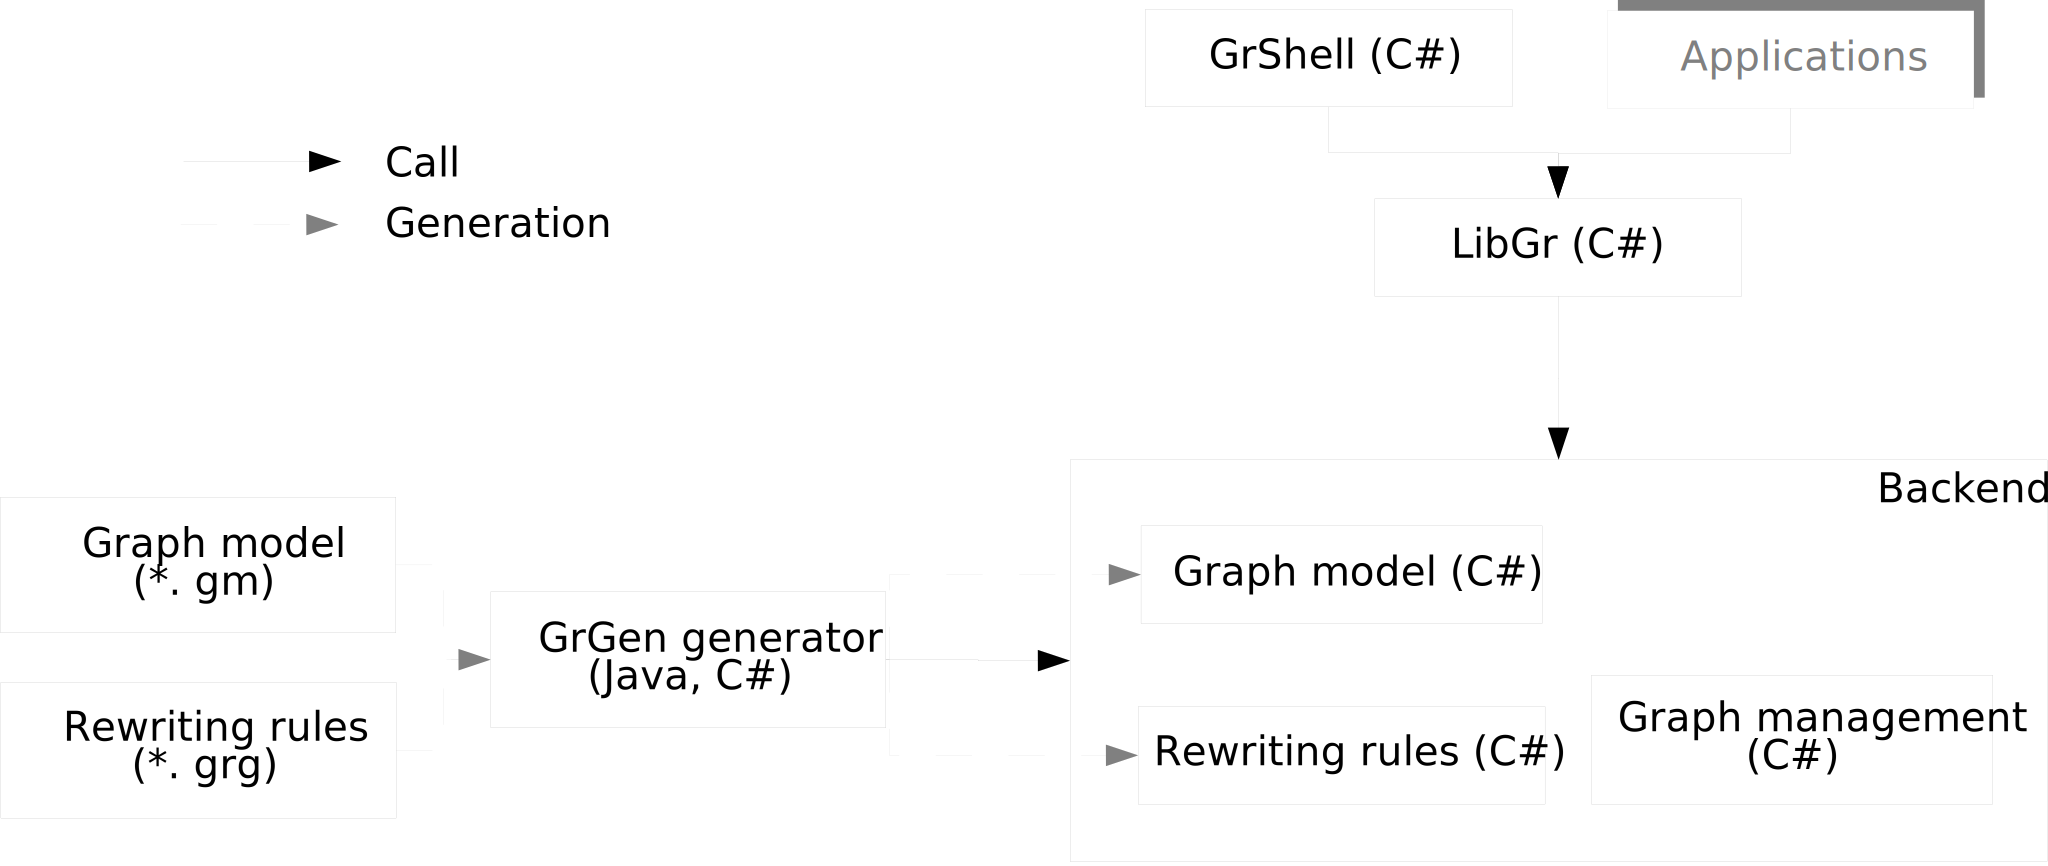
\includegraphics[width=\textwidth]{fig/Overview}
  \caption{\GrG\ system components \cite{kroll}}
  \label{figsys}
\end{figure}

\begin{table}[htbp]
  \begin{tabularx}{\linewidth}{|lX|} \hline
  bin & Contains the .NET assemblies, in particular GrGen.exe (the graph rewriting system generator), LGSPBackend.dll (a \GrG\ backend) and the shell GrShell.exe.  \\ 
  lib & Contains the \GrG\ generated assemblies (*.dll). \\
  specs & Contains the graph rewriting system source documents (*.gm and *.grg). \\ \hline
  \end{tabularx}
  \caption{\GrG\ directory structure}
  \label{dirstruc}
\end{table}

A graph rewriting system is defined by a rule set description file (*.grg) and one or more graph model description files (*.gm).\footnote{System, in this context, is not a CHO-like grammar rewriting system, but rather a set of interacting software components.} It is generated by GrGen.exe and can be used by \GrG\ applications such as GrShell. Figure \ref{process} shows the generation process.
\begin{figure}[htbp]
  \centering
  \includegraphics[width=\textwidth]{fig/process}
  \caption{Generating a graph rewriting system}
  \label{process}
\end{figure}

In general you have to distinguish carefully between a graph model (meta level), a host graph, a pattern graph and a rewriting rule. In \GrG\ pattern graphs are implicitly defined by rules, i.e.\ each rule defines its pattern. On the technical side, specification documents for a graph rewriting system can be available as source documents for graph models and rule sets (plain text *.gm and *.grg files) or as their translated .NET modules, either C\# source files or their compiled assemblies (*.dll).


\chapter{Graph Model Language}
\label{chapmodellang}
The key features of \GrG\ graph models from \cite{geiss}:

\begin{description}
\item[Types.] Nodes and edges can have types (classes). This is similar to common programming languages, except \GrG\ types have no concept of methods. 
\item[Attributes.] Nodes and edges can possess attributes. The set of attributes assigned to a node or edge is determined by its type. The attributes itself are typed, too.
\item[Inheritance.] Types (classes) can be composed by multiple inheritance. \emph{Node} and \emph{Edge} are built-in root types of node and edge types, respectively. Inheritance eases the specification of attributes, because subtypes inherit the attributes of their super types. Note that \GrG\ lacks a concept of overwriting. On a path in the type hierarchy graph from a type up to the built-in root type there must be exactly one declaration for each attribute identifier.
\item[Connection Assertions.] To specify that certain edge types should only connect specific nodes, we include connection assertions. Furthermore the number of outgoing and incoming edges can be constrained.
\end{description}

\begin{figure}[htbf]
\begin{example}\label{ex:model:map}
The following micro model of street maps gives a rough picture of the language:
\begin{grgen}
model Map;

enum resident {village = 500, town = 5000, city = 50000}

node class sight;

node class city {
	size: resident;
}

const node class metropolis extends city {
  river: string;
}  

abstract node class abandoned_city extends city;
node class ghost_town extends abandoned_city;

edge class street;
edge class trail extends street;
edge class highway extends street
    connect metropolis [+] -> metropolis [+]
{
    jam: boolean;
}
\end{grgen}
\end{example}
\end{figure}
In this chapter as well as in the \GrShell\ chapter \ref{chapgrshell} we use pieces of the example~\ref{ex:model:map} (the \texttt{Map} model) for further descriptions.

\section{Building Blocks}
\label{modelbb}

\begin{note}
The following syntax specifications make heavy use of syntax diagrams (also known as rail diagrams). Syntax diagrams provide a visualization of EBNF grammars. Follow a path along the arrows from left to right through a diagram to get a valid sentence (or sub sentence) of the language. Ellipses are terminals whereas rectangles are non-terminals. For further information on syntax diagrams see \cite{pascal}.
\end{note}
Basic elements of the \GrG\ graph model language are numbers and identifiers to denominate types, fields and the model itself. The \GrG\ graph model language is case sensitive.\\
\\
\emph{Ident}, \emph{IdentDecl}\\ \nopagebreak
A character sequence of arbitrary length consisting of letters, digits or underscores. The first character must not be a digit. \emph{Ident} and \emph{IdentDecl} differ in their role: while \emph{IdentDecl} is a \emph{defining} occurrence of an identifier, \emph{Ident} is a \emph{using} occurence. An \emph{IdentDecl} non-terminal can be annotated. See \ref{annotations} for annotations on declarations.\\
\\
\emph{NodeType}, \emph{EdgeType}, \emph{EnumType}\\ \nopagebreak
These are (semantic) specializations of Ident to restrict an identifier to a specific type.\\
\\
\emph{Number}\\ \nopagebreak
A sequence of digits. The sequence has to form a non-negative integer in decade system and will be internally stored in 32 bit two's complement representation.

\section{Type Declarations}
\begin{rail}
  GraphModel: 'model' IdentDecl ';' (() + TypeDeclaration);
\end{rail}
The graph model consists of its name \emph{IdentDecl} and type declarations defining specific node and edge types as well as enums.

\begin{rail}
  TypeDeclaration: EnumDeclaration | ClassDeclaration
\end{rail}
\emph{ClassDeclaration} defines a node or an edge. \emph{EnumDeclaration} defines an enum type for use as attribute of nodes or edges. Types do not need to be declared before they are used.

\begin{rail}
  EnumDeclaration: 'enum' IdentDecl lbrace ((IdentDecl (() | '=' IntExpr)) + ',') rbrace ;
\end{rail}
Defines an enum type.

\begin{example}
\begin{grgen}
enum Color {red, green, blue}
enum Resident {village = 500, town = 5000, city = 50000}
enum AsInC {a = 2, b, c = 1, d, e = Resident::village + c}
\end{grgen}
The semantics is as it is in C \cite{isoc}. So the examples hold $\text{red} = 0$, $a=d=2$, $b=3$, $c=1$ and $e=501$.
\end{example}

\begin{rail}  
  ClassDeclaration: (() | 'abstract') (() | 'const') (NodeClass | EdgeClass);
\end{rail}
Defines a new node type or edge type.\\
The keyword \texttt{abstract} indicates, that you can't instantiate graph elements of this type but rather you have to derive non-abstract types for graph elements. The abstract-property will not be inherited by subclasses.

\begin{example}
We adjust our map model and make \texttt{city} abstract:
\begin{grgen}
abstract node class city {
	size: int;
}
abstract node class abandoned_city extends city;
node class ghost_town extends abandoned_city;
\end{grgen}
You will be able to create nodes of type \texttt{ghost\_town}, but not of type \texttt{city} or \texttt{abandoned\_city}. However, nodes of type \texttt{ghost\_town} are also nodes of type \texttt{abandoned\_city} and of type \texttt{city} and they have got the attribute \texttt{size}.
\end{example}

The keyword \texttt{const} indicates, that rules may not write to attributes. See also \ref{replacepart}, \texttt{eval}. However, attributes are writable by \LibGr\ and \GrShell. This property will not be inherited by subclasses. If you want a subclass to have constant attributes, you have to set the \texttt{const} modifier explicitly.

\begin{rail}  
  NodeClass: 'node' 'class' IdentDecl (() | 'extends' (NodeType+',')) \\ 
    (';' | lbrace FieldDeclarations rbrace);
\end{rail}
Defines a new node type. Node types can inherit from other node types defined within the same file. If the \texttt{extends} clause is omitted, \emph{NodeType} will inherit from the built-in type \texttt{Node}. Optionally nodes can possess attributes (fields).

\begin{rail}    
  EdgeClass: 'edge' 'class' IdentDecl (() | 'extends' (EdgeType+',')) \\
    (() + ConnectAssertions) (';' | lbrace FieldDeclarations rbrace);
\end{rail}
Defines a new edge type. Edge types can inherit from other edge types defined within the same file. If the \texttt{extends} clause is omitted, \emph{EdgeType} will inherit from the built-in type \texttt{Edge}. Optionally edges can possess attributes (fields). A \emph{connection assertion} specifies that certain edge types should only connect specific nodes and -- moreover -- the number of outgoing and incoming edges can be constrained.

\begin{rail}  
  ConnectAssertions: 'connect' (NodeConstraint '->' NodeConstraint + ',');
  NodeConstraint: NodeType (() | '[' ('*' | '+' | Number | RangeConstraint) ']') ;
  RangeConstraint: Number ':' ('*' | Number) ;
\end{rail}
A connection assertion is described as a pair of node types, optionally together with a multiplicity. A corresponding edge may connect a node of the first node type or one of its subtypes (source) with a node of the second node type or one of its subtypes (destination). The multiplicity is a constraint on the out-degree and in-degree of the source and destination node type respectively. See \ref{graphcommands}, \texttt{validate}, for an example. Table \ref{multiplicities} describes the multiplicity definitions.
\begin{table}[htbp]
\begin{tabularx}{\linewidth}{|l|X|}\hline
	\texttt{[*]} & Number of edges the node is adjacent to is unbounded. The node must not be connected to any edge. This is the \textbf{default}.\\
	\texttt{[+]} & Number of edges the node is adjacent to is unbounded. At least one edge must be adjacent to nodes of that type.\\
	\texttt{[n:*]} & Number of edges the node is adjacent to is unbounded. At least $n$ edges must be adjacent to nodes of that type.\\ 
	\texttt{[n:m]} & At least $n$ edges must be adjacent to the nodes of that type, but at most $m$ edges may be adjacent to the nodes of that type ($m \geq n$ holds).\\
	\texttt{[n]} & Abbreviation for \texttt{[n:n]}. \\ \hline
\end{tabularx}
\caption{\GrG\ node constraint multiplicities concerning a specific pair of an edge type and a node type.}
\label{multiplicities}
\end{table}

\begin{rail}    
  FieldDeclarations: (() | IdentDecl ':' FieldType ';') + ;
  FieldType: PrimitiveType | EnumType ; 
\end{rail}
Defines a node or edge attribute. Possible types are \texttt{enum} and primitive types. See \ref{builtin} for a list of built-in primitive types.



\chapter{Rule Set Language}

The rule set language forms the core of \GrG. Rule files refer to one or multiple graph models and specify a set of (usually coherent) rewriting rules. The rule language covers the pattern specification and the replace / modify specification. Graph element's attributes can be re-evaluated during a rule application. The following rewriting rule from \cite{geiss} gives a rough picture of the language:
\begin{grgen}
actions SomeActions using SomeModel;

rule SomeRule {
  pattern {
    n1 : NodeTypeA;
    n2 : NodeTypeA;
    hom(n1, n2);
    n1 --> n2;
    n3: NodeTypeB;
    negative {
      n3 -e1:EdgeTypeA-> n1;
      if {n3.a1 == 42*n2.a1;}
    }
    negative {
      n4: Node \ (NodeTypeB);
      n3 -e1:EdgeTypeB->n4;
      if {typeof(e1) >= EdgeTypeA;}
    }
  }
  replace {
    n5: NodeTypeC<n1>;
    n3 -e1:EdgeTypeB-> n5;
    eval {
      n5.a3 = n3.a1*n1.a2;
    }
  }  
}
\end{grgen}
In this chapter we use pieces of \texttt{SomeRule} in further descriptions.

\section{Building Blocks}
\label{rulebb}

The \GrG\ rule set language is case sensitive. The language makes use of a couple of identifier specializations in order to denominate all the \GrG\ entities.\\
\\
\emph{Ident}, \emph{IdentDecl}\\ \nopagebreak
A character sequence of arbitrary length consisting of letters, digits or underscores. The first character must not be a digit. \emph{Ident} may be an identifier defined in a graph model (see \ref{modelbb}). \emph{Ident} and \emph{IdentDecl} differ in their role: while \emph{IdentDecl} is a \emph{defining} occurrence of an identifier, \emph{Ident} is a \emph{using} occurence. An \emph{IdentDecl} non-terminal can be annotated. See \ref{annotations} for annontations on declarations.
\\
\emph{ModelIdent}, \emph{TypeIdent}, \emph{NodeType}, \emph{EdgeType}\\
These are (semantic) specializations of Ident. \emph{TypeIdent} matches every type identifier, i.e. a node type, an edge type, an enum type or a primitive type. All the type identifiers are actually type \emph{expressions}. See \ref{typeexpressions} for the use of type expressions.\\

\begin{rail}
  ForwardEdge: '-' EdgeRefinement '->' ;
  ReverseEdge: '<-' EdgeRefinement '-' ;  
  EdgeRefinement: () | Ident | ':' EdgeType | IdentDecl ':' EdgeType (() | TypeConstraint | '<' Ident '>') ;
\end{rail}
In general edges are specified by \texttt{-->} or \texttt{<--}. Those edges are called \emph{anonymous}. For a more detailed specification use an edge refinement clause between the arrow dashes. Type constraints are allowed in the pattern part only. See \ref{typeexpressions}, \emph{TypeConstraint}. The \texttt{<>} operator retypes an edge. Retyping is allowed in the replace / modify part only. See \ref{replacepart}, \emph{Retyping}.

\section{Declarations}
\label{ruledecls}
\begin{rail}
  'actions' IdentDecl 'using' ((ModelIdent)+',') ';' \\ ((TestDeclaration | RuleDeclaration)+) ;
\end{rail}
A rule set consists of the underlying graph models and several rewriting rules. In case of multiple graph models \GrG\ use the union of the models. In this case beware of conflicting declarations.

\begin{rail}
  TestDeclaration: 'test' ActionSignature lbrace Pattern rbrace ;
  RuleDeclaration: 'rule' ActionSignature lbrace Pattern Replace rbrace ;
\end{rail}
Declares a single rewriting rule such as \texttt{SomeRule}. It consists of a pattern part (see \ref{patternpart}) together with its rewrite / modify part (see \ref{replacepart}). A test rule has no rewrite specification. It's intended to test wether (and maybe how many times) a pattern occurs.\\
\marginpar{\small \mbox{ }\\ \textbf{Example}}
{\small \\We define a test rule \texttt{SomeCond}}
\begin{grgen}
test SomeCond {
  pattern {
    n: SeldomNodeType;
  }
}
\end{grgen}
{\small and execute in \GrShell:}
\begin{grshell}
  grs SomeCond & SomeRule
\end{grshell}
{\small SomeRule will only be executed, if a node of type \texttt{SeldomNodeType} exists. For regular graph rewriting sequences in \GrShell\ see \ref{grsthings}.\\}

\begin{rail}  
  ActionSignature: IdentDecl (() | Parameters) (() | ':' ReturnTypes) ;
\end{rail}
The signature sets the name of a rewriting rule to \emph{IdentDecl}. Additionally you can provide parameters to the rule and specify return types.

\begin{rail}
  Parameters: '(' (IdentDecl ':' (NodeType | EdgeType) + ',') ')' ;
  ReturnTypes: '(' ((NodeType | EdgeType) + ',') ')' ;
\end{rail}
Parameters are treated as predefined graph elements for the pattern. Even if a supplied parameter value is undefined, it is treated as valid node or edge definition. So in any case a graph element of the specified type has to be matched. \\
The return types specify edge and node types of graph elements that are returned by the replace / modify part. If return types are specified, the \texttt{return} statement is mandatory. Otherwise no \texttt{return} statement may occur. If no pattern is found, the return values are undefined. See also \ref{replacepart}, \texttt{return}.\\
\marginpar{\mbox{ }\\ \small \textbf{Example}}
{\\ \small We extend \texttt{SomeRule} with a variable node to find, and we want it to return the rewritten graph elements \texttt{n5} and \texttt{e1}.}
\begin{grgen}
  rule SomeRuleExt(varnode: Node): (Node, EdgeTypeB) {
    pattern{
      n1: NodeTypeA;
      ...
    }
    replace {
      varnode;
      ...  
      return(n5, e1);
      eval {
        ...
\end{grgen}
{\small We don't define \texttt{varnode} within the pattern part, because this is already covered by the parameter specification itself.\\}

\section{Pattern Part}
\label{patternpart}
\begin{rail}
  Pattern: 'pattern' lbrace (()+PatternStatement) rbrace ;
\end{rail}
A pattern consists of zero, one or several pattern statements. All of the pattern statements must be fulfilled by a subgraph of the host graph, in order to form a match. Even stronger -- a graph element of the host graph, that is matched by a statement, is ``bound'', i.e.\ it can not be part of another pattern statement, unless you use the \texttt{hom} operator. An empty pattern always produces exactly one (empty) match.\\
Pattern statements may define variables for use by other pattern statements or replace statements. Such variables may be used before declaration.\\
\marginpar{\mbox{ }\\ \small \textbf{Note}} {\small \\ The application of a rule is not deterministic, specifically there may be more than one sub graph that matches the pattern and any of them may be selected.\\}

\begin{rail}  
  PatternStatement: 
    PatternGraphlet ';' |
    'hom' '(' (Ident + ',') ')' ';' |
    'negative' lbrace (()+PatternStatement) rbrace |
    'if' lbrace (BooleanExpr ';' +) rbrace |
    'return' '(' (Ident+',') ')' ';' ;
\end{rail}
The semantics of the various pattern statements:
\begin{description}
  \item[Pattern Graphlet.] Graphlets specify a connected subgraph, i.e.\ certain node types connected by certain edge types.
  \item[Isomorphic/Homomorphic Matching.] The \texttt{hom} operator specify the nodes or edges, that may be matched homomorphically. In contrast to the default isomorphic matching, the specified graph elements \emph{may} be matched to the same graph element in the host graph. Note that the graph elements shall have a common subtype. If the match is not isomorphic, than the elements will be mapped to a graph element of a common subtype.\\
  In our example \texttt{n1} and \texttt{n2} may be the same node. This is possible because they are of the  same type (\texttt{NodeTypeA}).
  \item[Negative Application Conditions (NACs).] With negative application conditions (keyword \texttt{negative}) we can specify graph patterns which forbid the application of a rule if any of them is present in the host graph (cf. \cite{adam}). NACs may not be nested. Variables defined within a NAC are not alive outside the NAC. Identifiers from surrounding scopes may be overwritten.\\
  In our example the second negative condition uses \texttt{n3} from the surrounding scope and defines \texttt{n4} and \texttt{e1}. We can safely reuse the variable name \texttt{e1} in the replace part.
  \item[Attribute Conditions.] The Java-like attribute conditions (keyword \texttt{if}) in the pattern part allows for further restriction of the applicability of a rule.
  \item[Return values.] The return statement is only allowed for \texttt{test} rules. Otherwise the \texttt{return} statement belongs to the replace part. See \ref{replacepart}, \emph{Return Values}.
\end{description}
Keep in mind that using type constraints or the \texttt{typeof} operator might be helpful. See \ref{typeexpressions} for further information.

\begin{rail}   
  PatternGraphlet: PatternNode (() | PatternContinuation) ;
  PatternContinuation: (ForwardEdge | ReverseEdge) PatternNode (() | PatternContinuation) ;
  PatternNode: Ident | 
    (() | IdentDecl) ':' NodeType (() | TypeConstraint) ; 
\end{rail}
A pattern graphlet is specified piecewise. Start with a \emph{PatternNode} in order to specify a node of type \emph{NodeType} (with respect to \emph{TypeConstraint}) and optionally construct a larger subgraph with several pattern continuations. \\
In our example the statement \texttt{n1 --> n2} is the node identifier \texttt{n1} followed by the pattern continuation \texttt{--> n2}.

\section{Replace / Modify Part}
\label{replacepart}
For the task of rewriting \GrG\ provides two different modes: a replace mode and a modify mode.
\begin{description}
  \item[Replace mode.] The semantics of this mode is to delete every graph element of the pattern that is not used (denoted) in the replace part, keep every graph element that is used and create all the additionally defined graph elements.\\
  In our example \texttt{SomeRuleExt} the nodes \texttt{varnode} and \texttt{n3} will be kept. The node \texttt{n1} is replaced by the node \texttt{n5} preserving \texttt{n1}'s edges. The anonymous edge instance between \texttt{n1} and \texttt{n2} only occurs in the pattern and therefore gets deleted.
  \item[Modify mode.] The modify mode can be regarded as a replace part in replace mode, where every pattern graph element is added (denoted) before the first replace statement. Additionally this mode supports the \texttt{delete} operator, that deletes every element given as an argument. Deletion takes place at last of all rewrite operations. Multiple deletion of the same graph element is allowed (but senseless) as well as deletion of just created elements (senseless, too).\\
\marginpar{\mbox{ } \\ \small \textbf{Example}} {\small \\ How might our example look in modify mode? We have to denominate the anonymous edge between \texttt{n1} and \texttt{n2} in order to delete it. The node \texttt{varnode} can be omitted. So we have}
\begin{grgen}
rule SomeRuleExtMod(varnode: Node): (Node, EdgeTypeB) {
  pattern {
    ...
    n1 -e0:Edge-> n2;
    ...
  }
  modify {
    n5 : NodeTypeC<n1>;
    n3 -e1:EdgeTypeB-> n5;
    delete(e0);
    eval {
      ...
\end{grgen}
\mbox{ }\\
\end{description}

\begin{rail}
  Replace: ('replace' | 'modify') lbrace (()+ReplaceStatement) rbrace ;
\end{rail}
Selects whether the replace mode or the modify mode is used. Several replace statements describe the transformation from the pattern subgraph to the destination subgraph.

\begin{rail}  
  ReplaceStatement: ReplaceGraphlet ';' |
    'delete' '(' (Ident + ',') ')' ';' |
    'eval' Evaluation |
    'return' '(' (Ident+',') ')' ';' ;
\end{rail}    
The semantics of the various pattern statements:
\begin{description}
  \item[Replace Graphlet.] Analogous to a pattern graphlet a specification of a connected subgraph. It's graph elements are either kept because they are elements of the pattern or added otherwise.
  \item[Deletion.] The \texttt{delete} operator is only supported by the modify mode. It deletes the specified pattern graph elements. Multiple occurrences of \texttt{delete} statements are allowed. Deletion statements are executed at last of all replace statements. Multiple deletion of the same graph element is allowed (but senseless) as well as deletion of just created elements (senseless, too).
  \item[Attribute Evaluation.] If a rule is applied, then the attributes of matched and inserted graph elements will be recalculated.
  \item[Return Values.] Graph elements of the replace part can be returned according to the return types in the signature (see \ref{ruledecls}, \texttt{ActionSignature}). The \texttt{return} statement may not occur multiple times. The values have to be in the same order as the corresponding return types in the signature.
  \item[Retyping.] Retyping enables us to keep all adjacent nodes and all attributes stemming from common super types of a graph element while changing its type. Retyping differs from a type cast: During replacement both of the graph elements are alive. Specifically both of them are available for evaluation. Furthermore the source and destination types must not be on a path in the directed type hierarchy tree, but are arbitrary.\\
The edge specification as well as \emph{ReplaceNode} supports retyping. In our example node \texttt{n5} is a retyped node stemming from node \texttt{n1}.
\end{description}    
    
\begin{rail}
  ReplaceGraphlet: ReplaceNode (() | ReplaceContinuation) ;
  ReplaceContinuation:  (ForwardEdge | ReverseEdge) ReplaceNode (() | ReplaceContinuation) ;    
\end{rail}
The same as \emph{PatternGraphlet}, but with \emph{ReplaceNode} instead of \emph{PatternNode}. The retyping operator for edges \texttt{<>} is allowed. See \ref{patternpart}, \emph{PatternGraphlet} and \emph{PatternContinuations}, for a description of the graphlet / continuation semantics.

\begin{rail}
  ReplaceNode: Ident | 
    (IdentDecl ':' NodeType (() | '<' Ident '>')) ;
\end{rail}
A single node that is either kept because it's a node of the pattern or added otherwise. \GrG\ supports \emph{retyping} of nodes by the \texttt{<>} operator.


\begin{rail}    
   Evaluation: lbrace ((Ident '.' Ident '=' Expression ';' )+) rbrace ;
\end{rail}
Several Evaluation parts are allowed within the replace part. Evaluation parts are executed before any graph elements get deleted. You can read (and write, although this doesn't make sense) attributes of deleted graph elements in modify mode or unmapped graph elements in replacement mode respectively.


\chapter{Types and Expressions}
\label{typeexpr}

In the following sections \emph{Ident} refers to an identifier of the graph model language (see section \ref{modelbb}) or the rule set language (see section \ref{rulebb}). \emph{TypeIdent} is an identifier of a node type or an edge type, \emph{NodeOrEdge} is an identifier of a node or an edge.

\section{Built-In Types}
\label{builtin}
Besides user-defined node types, edge types and enum types, GrGen supports the built-in \indexed{primitive types}\indexmainsee{built-in types}{primitive types} in table \ref{builtintypes}.
The exact type format is \indexed{backend} specific. 
The \indexed{LGSPBackend} maps the \GrG\ primitive types to the corresponding C\# primitive types.
\begin{table}[htbp]
\begin{tabularx}{\linewidth}{|l|X|}\hline
	\texttt{\indexed{boolean}} & Covers the values \texttt{true} and \texttt{false}. \\
	\texttt{\indexed{int}} & A signed integer with at least 32 bits. \\
	\texttt{\indexed{float}}, \texttt{\indexed{double}} & A floating-point number with single precision or double precision respectively. \\
	\texttt{\indexed{string}} & A character sequence of arbitrary length.\\ \hline
\end{tabularx}
\caption{\GrG\ built-in primitive types}
\label{builtintypes}
\end{table}
Table \ref{tabcasts} lists \GrG's implicit \indexed{type cast}s and the allowed explicit type casts. Of course you are free to express an implicit type cast by an explicit type cast as well as ``cast'' a type to itself, except for \indexed{enum type}s. The cast operator does never accept an enum type.
\begin{example}
  \texttt{myfloat = myint; mydouble = (float)myint; mystring = (string)mybool} is allowed, \\
  \texttt{myenum = (myenum)int; myfloat = mydouble; myint = (int)mybool} is forbidden.
\end{example}
\begin{table}[htbp]
  \centering
  \begin{tabular}[c]{|c|cccccc|} \hline
    \backslashbox{to}{from} & \texttt{enum} & \texttt{boolean} & \texttt{int} & \texttt{float} & \texttt{double} & \texttt{string}\\ \hline
    \texttt{enum} & $=$/--- & & & & & \\ 
    \texttt{boolean} & & $=$ & & & & \\
    \texttt{int} & \texttt{(int)} & & $=$ & \texttt{(int)} & \texttt{(int)} & \\
    \texttt{float} & \texttt{(float)} & & implicit & $=$ & \texttt{(float)} & \\
    \texttt{double} &  \texttt{(double)} & & implicit & implicit & $=$ & \\
    \texttt{string} & \texttt{(string)} & \texttt{(string)} & \texttt{(string)} & \texttt{(string)} & \texttt{(string)} & $=$ \\ \hline
  \end{tabular}
  \caption{\GrG\ type casts.}
  \label{tabcasts}
\end{table}

\section{Expressions}
\label{expressions}
\begin{rail}
  Expression: BoolExpr | IntExpr | FloatExpr | StringExpr | PrimaryExpr ;  
  BoolExpr: ((() | '!') PrimaryExpr) | (BoolExpr '?' BoolExpr ':' BoolExpr) | (BoolExpr BinBoolOperator BoolExpr) | (Expression CompareOperator Expression) | (TypeExpr CompareOperator TypeExpr);
\end{rail}
As in C \cite{Sch:1990:ANSIC}, \texttt{!}\ negates a boolean. 
Table \ref{tabboolops} lists the binary operators for boolean expressions. 
The \texttt{?}\ operator is a simple if-then-else: if the first \emph{BoolExpr} is evaluated to \texttt{true}, the operator returns the second \emph{BoolExpr}, otherwise it returns the third \emph{BoolExpr}.
The \emph{CompareOperator} is one of the following operators:
\[ \texttt{<} \;\;\;\;\; \texttt{<=} \;\;\;\;\; \texttt{==} \;\;\;\;\; \texttt{!=} \;\;\;\;\; \texttt{>=} \;\;\;\;\; \texttt{>} \]
These operators are supported by enum types, \texttt{int} types, and \texttt{float}/\texttt{double} types.
\texttt{String} types and \texttt{boolean} types support only the \texttt{==} and the \texttt{!=} operators.
Table \ref{compandtypes} describes the semantics of compare operators on \indexed{type expression}s.
The \emph{BinBoolOperator} is one of the operators in table \ref{tabboolops}.
\begin{table}[htbp]
\label{compandtypes} 
  \centering
  \begin{tabularx}{\linewidth}{|l|X|} \hline
    \texttt{A == B} & True, iff $A$ and $B$ are identical. Different types in a type hierarchy are \emph{not} identical. \\
    \texttt{A != B} & True, iff $A$ and $B$ are not identical. \\
    \texttt{A < B} & True, iff $A$ is a supertype of $B$, but $A$ and $B$ are not identical. \\
    \texttt{A > B} & True, iff $A$ is a subtype of $B$, but $A$ and $B$ are not identical. \\
    \texttt{A <= B} & True, iff $A$ is a supertype of $B$ or $A$ and $B$ are identical. \\
    \texttt{A >= B} & True, iff $A$ is a subtype of $B$ or $A$ and $B$ are identical. \\ \hline
  \end{tabularx}
  \caption{Compare operators on type expressions}
  \label{compandtypes}
\end{table}
\begin{note}
  \texttt{A < B} corresponds to the direction of the arrow in an \indexed{UML class diagram}.
\end{note}

\begin{table}[htbp] 
  \centering
  %\begin{tabularx}{0.45\linewidth}{|ll|} \hline
  \begin{tabular}[c]{|lp{0.6\linewidth}|} \hline
    \begin{tabular}[c]{l} \texttt{\^} \end{tabular} & \begin{tabular}[c]{l} Logical XOR. True, iff either the first or the second \\ Boolean expression is true. \end{tabular} \\ \hline
    \begin{tabular}[c]{l} \texttt{\&\&} \\ \texttt{||} \end{tabular} & \begin{tabular}[c]{l} Logical AND and OR. Lazy evaluation. \end{tabular}\\ \hline
    \begin{tabular}[c]{l} \texttt{\&} \\ \texttt{|} \end{tabular} & \begin{tabular}[c]{l} Logical AND and OR. Strict evaluation. \end{tabular}\\ \hline
  \end{tabular}
  \caption{Binary boolean operators, in ascending order of precedence}\indexmain{order of precedence}\indexmainsee{precedence}{order of precedence}
  \label{tabboolops}
\end{table}

\begin{rail}
  IntExpr: ((() | '+' | '-' | tilde) PrimaryExpr) | (BoolExpr '?' IntExpr ':' IntExpr) | (IntExpr BinIntOperator IntExpr);
\end{rail}
The $\sim$ operator is the bitwise complement. 
That means every bit of an integer value will be flipped. 
The \texttt{?}\ operator is a simple if-then-else: if the \emph{BoolExpr} is evaluated to \texttt{true}, the operator returns the first \emph{IntExpr}, otherwise it returns the second \emph{IntExpr}. 
The \emph{BinIntOperator} is one of the operators in table \ref{tabbinops}.
\begin{table}[htbp] 
  \centering
  %\begin{tabularx}{0.45\linewidth}{|ll|} \hline
  \begin{tabular}[c]{|lp{0.6\linewidth}|} \hline
    \begin{tabular}[c]{l} \texttt{\^} \\ \texttt{\&} \\ \texttt{|} \end{tabular} & \begin{tabular}[c]{l} Bitwise XOR, AND and OR \end{tabular} \\ \hline
    \begin{tabular}[c]{l} \texttt{\mbox{<}\mbox{<}} \\ \texttt{\mbox{>}\mbox{>}} \\ \texttt{\mbox{>}\mbox{>}\mbox{>}} \end{tabular} & \begin{tabular}[c]{l} Bitwise shift left, bitwise shift right and \\ bitwise shift right preserving the sign \end{tabular}\\ \hline
    \begin{tabular}[c]{l} \texttt{+} \\ \texttt{-} \end{tabular} & \begin{tabular}[c]{l} Addition and subtraction \end{tabular}\\ \hline
    \begin{tabular}[c]{l} \texttt{*} \\ \texttt{/} \\ \texttt{\%} \end{tabular} & \begin{tabular}[c]{l}Multiplication, integer division and modulo \end{tabular} \\ \hline
  \end{tabular}
  \caption{Binary integer operators, in ascending order of precedence}\indexmain{order of precedence}
  \label{tabbinops}
\end{table}

\begin{rail}  
  FloatExpr: ((() | '+' | '-') PrimaryExpr) | (BoolExpr '?' FloatExpr ':' FloatExpr) | (FloatExpr BinFloatOperator FloatExpr);
\end{rail} 
The \texttt{?}\ operator is a simple if-then-else: if the \emph{BoolExpr} is evaluated to \texttt{true}, the operator returns the first \emph{FloatExpr}, otherwise it returns the second \emph{FloatExpr}.
The \emph{BinFloatOperator} is one of the operators in table \ref{tabfloatbinops}.
\begin{table}[htbp] 
  \centering
  %\begin{tabularx}{0.45\linewidth}{|ll|} \hline
  \begin{tabular}[c]{|ll|} \hline
    \begin{tabular}[c]{l} \texttt{+} \\ \texttt{-} \end{tabular} & \begin{tabular}[c]{l} Addition and subtraction \end{tabular}\\ \hline
    \begin{tabular}[c]{l} \texttt{*} \\ \texttt{/} \\ \texttt{\%} \end{tabular} & \begin{tabular}[c]{l}Multiplication, division and modulo \end{tabular} \\ \hline
  \end{tabular}
  \caption{Binary float operators, in ascending order of precedence}\indexmain{order of precedence}
  \label{tabfloatbinops}
\end{table}
\begin{note}
The \texttt{\%} operator works analogous to the integer modulo operator. For instance \texttt{4.5 \% 2.3 == 2.2}. \GrG\ implements the Java semantics. 
\end{note}

\begin{rail}
  StringExpr: PrimaryExpr | StringExpr '+' StringExpr;
\end{rail}
The operator \texttt{+} concatenates two strings.

\begin{rail} 
  PrimaryExpr: '(' ('int' | 'float' | 'double' | 'string') ')' PrimaryExpr | '(' Expression ')' | (NodeOrEdge '.' Ident) | (EnumType '::' Ident) | Constant;
  Constant: Number | HexNumber | QuotedText | 'true' | 'false';
\end{rail}
\begin{description}
  \item[Number.] Is an \texttt{int}, \texttt{float} or \texttt{double} constant in decimal notation.
  \item[HexNumber.] Is an \texttt{int} constant in hexadecimal notation starting with \texttt{0x}.
  \item[QuotedText.] Is a string constant. It consists of a sequence of characters, enclosed by double quotes.
\end{description}

\section{Type Related Conditions}\indexmain{type expression}
\label{typeexpressions}

\begin{rail}
  TypeExpr: TypeIdent | 'typeof' '(' NodeOrEdge ')' ;
\end{rail}\indexmain{\texttt{typeof}}
A type expression identifies a type (and---in terms of matching---also its subtypes). A type expression is either a type identifier itself or the type of a graph element.
\begin{example}
The following rule will add a reverse edge to a one-way street.
\begin{grgen}
rule oneway {
    pattern {
        a:Node -x:street-> y:Node;
        negative{
            y -:typeof(x)-> a;
        }
    } 
    replace {
        a -x-> y;
        y -:typeof(x)-> a;
    }
}
\end{grgen}
Remember that we have several subtypes of \texttt{street}. By the aid of the \texttt{typeof} operator, the reverse edge will be automatically typed correctly (the same type as the one-way edge). This behavior is not possible without the \texttt{typeof} operator.
\end{example}

\begin{rail}
  TypeConstraint: backslash '(' (TypeExpr + '+')  ')' ; 
\end{rail}
A \indexed{type constraint} is used to exclude parts of the \indexed{type hierarchy}. The operator \texttt{+} is used to create a union of its operand types. So the following pattern statements are identical:\\
\begin{center}
\begin{tabular}[c]{lll}
\begin{tabular}{|l|}\hline\texttt{x:T \char"5C\ (T1 + T2);}\\\hline\end{tabular} && 
  \begin{tabular}{|l|}\hline\texttt{x:T;} \\ \texttt{if \{!(\emph{typeof}(x) == T1) \&\& !(\emph{typeof}(x) == T2)\}}\\\hline\end{tabular}
\end{tabular}
\end{center}
\begin{example}
\begin{tabularx}{\linewidth}{cX}
  \parbox{0.25\linewidth}{\includegraphics[width=\linewidth]{fig/hierarchy}} &
  \parbox{\linewidth}{The expression \texttt{A\char"5C (C+E)} applied to the type hierarchy on the left side covers $A$ and $B$.}
\end{tabularx}
\end{example}

\section{Annotations}\indexmain{annotation}
\label{annotations}

Identifier \indexed{definition}s can be annotated by \indexedsee{pragma}{annotation}s. Annotations are key-value pairs.
\begin{rail}
  IdentDecl: Ident (() | '[' (Ident '=' Constant + ',') ']');
\end{rail}
Although you can use any key-value pairs between the brackets, only the identifier \indexed{\texttt{prio}} has an effect so far.
\begin{table}[htbp]
\begin{tabularx}{\linewidth}{|lllX|} \hline
  \textbf{Key} & \textbf{Value Type} & \textbf{Applies to} & \textbf{Meaning} \\ \hline
  \texttt{prio} & int & node, edge & Changes the ranking of a graph element for \indexed{search plan}s. The default is \texttt{prio}=1000. Graph elements with high values are likely to appear prior to graph elements with low values in search plans.\\ \hline
\end{tabularx}
\caption{Annotations}
\label{tabannotations}
\end{table}
\begin{example}
We search the pattern \texttt{v:NodeTypeA -e:EdgeType-> w:NodeTypeB}. We have a host graph with about 100 nodes of \texttt{NodeTypeA}, 1,000 nodes of \texttt{NodeTypeB} and 10,000 edges of \texttt{EdgeType}. Furthermore we know that between each pair of \texttt{NodeTypeA} and \texttt{NodeTypeB} there exists at most one edge of \texttt{EdgeType}. \GrG\ can use this information to improve the initial search plan, if we adjust the pattern like \texttt{v[prio=10000]:NodeTypeA -e[prio=5000]:EdgeType-> w:NodeTypeB}.
\end{example}


\chapter{GrShell Language}\indexmain{GrShell}
\label{chapgrshell}
\TODO{Explain the debugger in its own subsection, XGRS, new syntax}
\GrShell\ is a \indexedsee{shell}{GrShell} application of \LibGr\indexmain{libGr}. 
It belongs to \GrG's standard equipment. \GrShell\ is capable of creating, manipulating, and dumping graphs as well as performing and debugging graph rewriting.
The \GrShell\ provides a line oriented scripting language. 
\GrShell\ scripts are structured by simple statements separated by line breaks.

\section{Building Blocks}

\GrShell\ is \indexed{case sensitive}. 
A \indexed{comment} starts with a \indexed{\texttt{\#}} and is terminated by end-of-line or end-of-file. 
Any text left of the \texttt{\#} will be treated as a statement.
The following items are required for representing text, numbers, and rule parameters.\\
\\
\emph{Text}\\
May be one of the following:
\begin{itemize}
  \item A non-empty character sequence consisting of letters, digits, and underscores. The first character must not be a digit.
  \item Arbitrary text enclosed by double quotes (\texttt{""}).
  \item Arbitrary text enclosed by single quotes (\texttt{''}).
\end{itemize}
\mbox{ }\\
\emph{Number}\\
Is an \texttt{int} or \texttt{float} constant in decimal notation (see also Section~\ref{builtin}).

\begin{rail} 
 Parameters : Text + ',' ;
 SpacedParameters: Text + ; 
\end{rail}\ixnterm{Parameters}\ixnterm{SpacedParameters}

In order to describe the commands more precisely, the following (semantic) specializations of \emph{Text} are defined:
\begin{description}
  \item[Filename]A fully qualified file name without spaces (e.g.\ \texttt{/Users/Bob/amazing\textunderscore file.txt}) or a single quoted or double quoted fully qualified file name that may contain spaces (\texttt{"/Users/Bob/amazing file.txt"}).
  \item[Variable] Identifier of a variable that contains a graph element. 
  \item[NodeType, EdgeType] Identifier of a node type resp.\ edge type defined in the model of the current graph.
  \item[AttributeName] Identifier of an attribute.
  \item[Graph] Identifies a graph by its name.
  \item[Action] Identifies a rule by its name.
  \item[Color] One of the following \indexed{color} identifiers: \texttt{Black}, \texttt{Blue}, \texttt{Green}, \texttt{Cyan}, \texttt{Red}, \texttt{Purple}, \texttt{Brown}, \texttt{Grey}, \texttt{LightGrey}, \texttt{LightBlue}, \texttt{LightGreen}, \texttt{LightCyan}, \texttt{LightRed}, \texttt{LightPurple}, \texttt{Yel\-low}, \texttt{White}, \texttt{DarkBlue}, \texttt{DarkRed}, \texttt{DarkGreen}, \texttt{DarkYellow}, \texttt{DarkMagenta}, \texttt{DarkCyan}, \texttt{Gold}, \texttt{Lilac}, \texttt{Turquoise}, \texttt{Aquamarine}, \texttt{Khaki}, \texttt{Pink}, \texttt{Orange}, \texttt{Orchid}. These are the same color identifiers as in \indexed{VCG}/\yComp\ files (for a VCG definition see~\cite{vcg}).
\end{description}
\makeatletter
\begin{rail}
  GraphElement: Text | ('@' '(' Text ')')
\end{rail}\indexmain{\texttt{"@}}\ixnterm{GraphElement}
\makeatother
The elements of a graph (nodes and edges) can be accessed both by their \indexed{variable} identifier and by their \newterm{persistent name} specified through a constructor (see Section~\ref{mani}).
The specializations \emph{Node} and \emph{Edge} of \emph{GraphElement} require the corresponding graph element to be a node or an edge respectively.
\begin{example}
\label{persistentex} 
We insert a node, \indexed{anonymous}ly and with a \indexed{constructor} (see also Section~\ref{mani}):
\begin{grshell}
> new graph "../lib/lgsp-TuringModel.dll" G
New graph "G" of model "Turing" created.
  
# insert an anonymous node... 
# it will get a persistent pseudo name
> new :State  
New node "$0" of type "State" has been created.
> delete node @("$0")
  
# and now with constructor
> new v:State($=start) 
new node "start" of type "State" has been created.
# Now we have a node named "start" and a variable v assigned to "start"
\end{grshell}
\end{example}
\begin{note}
Persistent names belong to a specific graph whereas variables belong to the current \GrShell\ environment. Persistent names will be saved (\texttt{save graph\dots}, see Section~\ref{outputcmds}) and, if you visualize a graph (\texttt{dump graph\dots}, see Section~\ref{outputcmds}), graph elements will be \indexed{label}ed with their persistent names. Persistent names have to be unique for a graph.
\end{note}

\begin{rail}
  Variable '=' GraphElement   
\end{rail}
Assigns the variable or persistent name \emph{GraphElement} to \emph{Variable}. If \emph{Variable} has not been defined yet, it will be defined implicitly. As usual for scripting languages, variables have neither static types nor declarations.

\section{\GrShell\ Commands}
This section describes the \GrShell\ commands\ixnterm{Command}. Commands are assembled from basic elements. 
As stated before commands are terminated by line breaks. Alternatively commands can be terminated by the \indexed{\texttt{;;}} symbol.
Like an operating system shell, the \GrShell\ allows you to span a single command over $n$ lines by terminating the first $n-1$ lines with a \indexed{backslash}.  
\begin{rail}
  Script: ((Command ('<line break>' | ';;'))+) '<end of file>' ;
\end{rail}\ixnterm{Script}

\subsection{Common Commands}
\label{commcommands}
\begin{rail}
  'help'
\end{rail}\ixkeyw{help}
Displays an information message describing supported commands. 

\begin{rail}
  'quit' | 'exit'
\end{rail}\ixkeyw{quit}\ixkeyw{exit}
Quits \GrShell. If \GrShell\ is opened in debug mode, a currently active graph viewer (such as \yComp) will be closed as well.

\begin{rail}
  'select' 'backend' Filename ( ( ) | ':' Parameters )
\end{rail}\ixkeyw{select}\ixkeyw{backend}
Selects a \indexed{backend} that handles graph and rule representation. \emph{Filename} has to be a .NET assembly (e.g.\ \texttt{\indexed{lgspBackend.dll}}).
Comma-separated \indexed{parameter}s can be supplied optionally; if so, the backend must support these parameters.
By default the LGSPBackend is used.

\begin{rail}
  'show' 'backend'
\end{rail}\nopagebreak\ixkeyw{show}\ixkeyw{backend}
List all the parameters supported by the currently selected backend. The parameters can be provided to the \texttt{select backend} command.

\begin{rail}
  'include' Filename
\end{rail}\ixkeyw{include}
Executes the \GrShell\ script\indexmain{graph rewrite script} \emph{Filename}. A \GrShell\ script is just a plain text file containing \GrShell\ commands. They are treated as they would be entered interactively, except for parser errors. If a parser error occurs, execution of the script will stop immediately.

\begin{rail}
  'debug' ( 'enable' | 'disable' )
\end{rail}\ixkeyw{debug}\ixkeyw{enable}\ixkeyw{disable}
Enables and disables the \indexed{debug mode}. The debug mode shows the current working graph in a \yComp\ window. All changes to the working graph are tracked by \yComp\ immediately.  

\begin{rail}
  'debug' 'set' 'layout' (() | Text) ;
\end{rail}\ixkeyw{debug}\ixkeyw{set}\ixkeyw{layout}
Sets the default graph \indexed{layout algorithm} to \emph{Text}. If \emph{Text} is omitted, a list of available layout algorithms is displayed. See Section~\ref{tools:ycomp} on \yComp\ layouters.

\begin{rail}
  'echo' Text
\end{rail}\ixkeyw{echo}
Prints \emph{Text} onto the \GrShell\ command prompt.

\begin{rail}
  '!' CommandLine
\end{rail}\indexmain{\texttt{"!}}
\emph{CommandLine}\indexmain{command line} is an arbitrary text, the operating system attempts to execute.
\begin{example}
On a Linux machine you might execute
\begin{grshell}
!sh -c "ls | grep stuff"
\end{grshell}
\end{example}

\subsection{Graph Commands}
\label{graphcommands}

\begin{rail}
  'new' 'graph' Filename Text 
\end{rail}\ixkeyw{new}\ixkeyw{graph}
Creates a new graph with the model specified in \emph{Filename}\indexmain{graph model}. Its name is set to \emph{Text}. The model file can be either source code (e.g.\ \texttt{turing\textunderscore machineModel.cs}) or a .NET assembly (e.g.\ \texttt{lgsp-turing\textunderscore machineModel.dll}).

\begin{rail}
  'open' 'graph' Filename Text
\end{rail}\ixkeyw{open}\ixkeyw{graph}
Opens the graph \emph{Text} stored in the backend. However, the \emph{LGSPBackend} doesn't support \indexed{persistent graph}s. The \emph{LGSPBackend} is the only backend so far. Therefore this command is currently useless.

\begin{rail}
  'show' 'graphs'
\end{rail}\ixkeyw{show}\ixkeyw{graph}
Displays a list of currently available graphs.

\begin{rail}
  'select' 'graph' Graph
\end{rail}\ixkeyw{select}\ixkeyw{graph}
Selects the current \indexed{working graph}. This graph acts as \emph{\indexed{host graph}} for graph rewrite sequences (see also Sections~\ref{ov:whatsallabout} and~\ref{grsthings}). Though you can define multiple graphs, only one graph can be the active ``working graph''.

\begin{rail}
  'clear' 'graph' (() | Graph)
\end{rail}\ixkeyw{clear}\ixkeyw{graph}
Deletes all graph elements of the current working graph resp.\ the graph \emph{Graph}.

\begin{rail}
  'delete' 'graph' Graph
\end{rail}\ixkeyw{delete}\ixkeyw{graph}
Deletes the graph \emph{Graph} from the backend storage.

\begin{rail}
  'validate' ( ( ) | 'strict' )
\end{rail}\ixkeyw{validate}\ixkeyw{strict}
Validates\indexmain{validate} if the current working graph fulfills the \indexed{connection assertion}s specified in the corresponding graph model. The \emph{strict} mode additionally requires all the edges of the working graph to be specified in order to get a ``valid''. Otherwise edges between nodes without specified constraints are ignored.\\
\begin{example}
We reuse a simplified version of the road map model from chapter~\ref{chapmodellang}:
\begin{grgen} 
model Map;

node class city;
node class metropolis;

edge class street;
edge class highway
      connect metropolis [+] -> metropolis [+];
\end{grgen}
The node constraint on \emph{highway} requires all the metropolises to be connected by highways. Now have a look at the following graph:
\begin{center}
  \fbox{\includegraphics[width=8.5cm]{fig/map}}
\end{center}

This graph is valid but not strict valid.
\begin{grshell} 
> validate
The graph is valid.
> validate strict
The graph is NOT valid:
  CAE: city "Eppstein" -- highway "A3" --> metropolis "Frankfurt" not specified
  CAE: metropolis "Karlsruhe" -- street "trail" --> metropolis "Frankfurt" not specified
>
\end{grshell}
\end{example}

\begin{rail}
  'custom' 'graph' ( ( ) | SpacedParameters )
\end{rail}\ixkeyw{custom}\ixkeyw{graph}
Executes a command specific to the current backend. If \emph{SpacedParameters} is omitted, a list of available commands will be displayed (for the LGSP backend see Sections~\ref{custom}).

\subsection{Graph Manipulation Commands}
\label{mani}
Graph manipulation commands alter existing graphs including creating and deleting graph elements and setting attributes.

\begin{rail}
  Constructor : '(' (() | (dollar '=' Text (() | ',' Attributes) | Attributes)) ')';
  Attributes : AttributeName '=' (Text | Number) + ',' ;
\end{rail}\indexmain{\texttt{\$}}\ixnterm{Constructor}\ixnterm{Attributes}
A \indexed{constructor} is used to initialize a new graph element (see \texttt{new \dots} below). A comma separated list of \indexed{attribute} declarations is supplied to the constructor. Available attribute names are specified by the graph model of the current working graph. All the undeclared attributes will be initialized with \indexed{default value}s, depending on their type (int $\leftarrow$ \texttt{0}, enum $\leftarrow$ unspecified; boolean $\leftarrow$ \texttt{false}; float, double $\leftarrow$ \texttt{0.0}; string $\leftarrow$ \texttt{""}).\\
The \texttt{\$} is a special attribute name: a unique identifier of the new graph element. This identifier is also called \newterm{persistent name} (see Example~\ref{persistentex}). This name can be specified by a constructor only.

\begin{rail}
  'new' (() | Text) (() | ':' NodeType (() | Constructor))
\end{rail}\ixkeyw{new}
Creates a new node within the current graph. Optionally a variable \emph{Text} is assigned to the new node. If \emph{NodeType} is supplied, the new node will be of type \emph{NodeType} and attributes can be initialized by a constructor. Otherwise the node will be of the base node class type \emph{Node}.
\begin{note}
The \GrShell\ can reassign \indexed{variable}s. 
This is in contrast to the rule language (chapter~\ref{chaprulelang}), where we use \emph{names}\indexmain{name}.
\end{note}

\begin{rail}
  'new' Node '-' (()|Text) \\ (() | ':' EdgeType (() | Constructor)) '->' Node
\end{rail}\ixkeyw{new}
Creates a new edge within the current graph between the specified nodes, directed towards the second \emph{Node}. Optionally a variable \emph{Text} is assigned to the new edge. If \emph{EdgeType} is supplied, the new edge will be of type \emph{EdgeType} and attributes can be initialized by a constructor. Otherwise the edge will be of the base edge class type \emph{Edge}.

\begin{rail}
  GraphElement '.' AttributeName '=' (Text | Number) ;
\end{rail}
Set the \indexed{attribute} \emph{AttributeName} of the graph element \emph{GraphElement} to the value of \emph{Text} or \emph{Number}.

\begin{rail}
  'delete' 'node' Node
\end{rail}\ixkeyw{delete}\ixkeyw{node}
Deletes the node \emph{Node} from the current graph. Incident edges will be deleted as well.

\begin{rail}
  'delete' 'edge' Edge
\end{rail}\ixkeyw{delete}\ixkeyw{edge}
Deletes the edge \emph{Edge} from the current graph.
  
\subsection{Graph Query Commands}

\begin{rail}
  'show' (() | 'num') ('nodes' (() | (() | 'only') NodeType) | 'edges' (() | (() | 'only') EdgeType))
\end{rail}\ixkeyw{show}\ixkeyw{num}\ixkeyw{nodes}\ixkeyw{edges}\ixkeyw{only}
Gets the \indexed{persistent name}s and the types of all the nodes/edges of the current graph. 
If a node type or edge type is supplied, only elements compatible to this type are considered. 
The \texttt{only} keyword excludes subtypes. Nodes/edges without persistent names are shown with a pseudo-name.
If the command is specified with \texttt{num}, only the number of nodes/edges will be displayed.

\begin{rail}
  'show' ('node' | 'edge') 'types'
\end{rail}\ixkeyw{show}\ixkeyw{node}\ixkeyw{edge}
Gets the node/edge types of the current graph model.

\begin{rail}
'show' ('node' ('super' | 'sub') 'types' NodeType | 'edge' ('super' | 'sub') 'types' EdgeType)
\end{rail}\ixkeyw{show}\ixkeyw{node}\ixkeyw{edge}\ixkeyw{super}\ixkeyw{sub}\indexmain{inheritance}
Gets the inherited/descendant types of \emph{NodeType}/\emph{EdgeType}.

\begin{rail}
  'show' ('node' 'attributes' (() | (() | 'only') NodeType) | 'edge' 'attributes' (() | (() | 'only') EdgeType))
\end{rail}\ixkeyw{show}\ixkeyw{node}\ixkeyw{edge}\ixkeyw{only}
Gets the available node/edge \indexed{attribute} types. If \emph{NodeType}/\emph{EdgeType} is supplied, only attributes defined in \emph{NodeType}/\emph{EdgeType} are diplayed. The \texttt{only} keyword excludes inherited attributes.\\
\begin{note}
The \texttt{show nodes/edges attributes\dots} command covers types and \emph{inherited} types. This is in contrast to the other \texttt{show\dots} commands where types and \emph{sub}types are specified or the direction in the type hierarchy is specified explicitly, respectively.
\end{note}

\begin{rail}
 'show' ('node' Node | 'edge' Edge)
\end{rail}\ixkeyw{show}\ixkeyw{node}\ixkeyw{edge}
Gets the attribute types and values of a specific graph element.

\begin{rail}
  'show' GraphElement '.' AttributeName
\end{rail}\ixkeyw{show}
Gets the value of a specific attribute.

\begin{rail}
  'node' 'type' Node 'is' Node | 'edge' 'type' Edge 'is' Edge
\end{rail}\ixkeyw{node}\ixkeyw{edge}\ixkeyw{type}\ixkeyw{is}
Gets the information whether the first element is \indexed{type-compatible}\indexmainsee{compatible types}{type-compatible} to the second element.

\subsection{Graph Output Commands}
\label{outputcmds}

\begin{rail}
  'save' 'graph' Filename
\end{rail}\ixkeyw{save}\ixkeyw{graph}
Dumps\indexmain{dumping graph} the current graph as \GrShell\ script\indexmain{graph rewrite script} into \emph{Filename}. The created script includes
\begin{itemize}
  \item selecting the backend
  \item creating all nodes and edges
  \item restoring the persistent names (see Section~\ref{mani})
\end{itemize}
but not necessarily using the same commands you typed in during construction. 
Such a script can be loaded and executed by the \texttt{include} command (see Section~\ref{commcommands}).

\begin{rail}
  'show' 'graph' Filename (() | Text)
\end{rail}\ixkeyw{show}\ixkeyw{graph}
Dumps the current graph as \indexed{VCG} formatted file into a temporary file. \emph{Filename} specifies an executable. The temporary VCG file will be passed to \emph{Filename} as last parameter. Additional parameters, such as program options, can be specified by \emph{Text}. If you use \yComp\footnote{See Section~\ref{tools:ycomp}.}\indexmain{yComp} as executable, this may look like
\begin{center}
  \includegraphics[width=0.75\linewidth]{fig/showgraph}
\end{center}  
The temporary file will be deleted, when the application \emph{Filename} is terminated if \GrShell\ is still running at this time.

\begin{rail}
  'dump' 'graph' Filename
\end{rail}\ixkeyw{dump}\ixkeyw{graph}
Dumps the current graph in \indexed{VCG} format into the file \emph{Filename}.\\

\paragraph{Visualization Styles}
The following commands control the style of the VCG output. This affects \texttt{dump graph}, \texttt{show graph}, and \texttt{enable debug}. 
\begin{rail}
  'dump' 'set' 'node' (() | 'only') NodeType \\ (('color' | 'textcolor' | 'bordercolor') Color | 'shape' Text) ;
\end{rail}\ixkeyw{dump}\ixkeyw{set}\ixkeyw{node}\ixkeyw{only}\ixkeyw{color}\ixkeyw{textcolor}\ixkeyw{bordercolor}\ixkeyw{shape}
Sets the \indexed{color}, text color, border color, or the shape of the nodes of type \emph{NodeType} and all of its subtypes. The keyword \texttt{only} excludes the subtypes. The following shapes are supported: \texttt{box}, \texttt{triangle}, \texttt{circle}, \texttt{ellipse}, \texttt{rhom}, \texttt{hexagon}, \texttt{trapeze}, \texttt{uptrapeze}, \texttt{lparallelogram}, \texttt{rparallelogram}. Those are shape names of \yComp\ (for a VCG definition see~\cite{vcg}).

\begin{rail}
  'dump' 'set' 'edge' (() | 'only') EdgeType ('color' | 'textcolor') Color ;
\end{rail}\ixkeyw{dump}\ixkeyw{set}\ixkeyw{edge}\ixkeyw{only}\ixkeyw{color}\ixkeyw{textcolor}
Sets the color or text color of the edges of type \emph{EdgeType} and all of its subtypes. The keyword \texttt{only} excludes the subtypes.

\begin{rail}
  'dump' 'add' 'node' (() | 'only') NodeType 'exclude' ;
\end{rail}\ixkeyw{dump}\ixkeyw{add}\ixkeyw{node}\ixkeyw{only}\ixkeyw{exclude}
Excludes nodes of type \emph{NodeType} and all of its subtypes as well as their incident edges from output. The keyword \texttt{only} excludes the subtypes, i.e.\ subtypes of \emph{NodeType} are dumped.

\begin{rail}
  'dump' 'add' 'node' NodeType 'group' ;
\end{rail}\ixkeyw{dump}\ixkeyw{add}\ixkeyw{node}\ixkeyw{group}
Declares \emph{NodeType} and subtypes of \emph{NodeType} as \indexed{group node} type. All the differently typed nodes that point to a node of type \emph{NodeType} (i.e.\ there is a directed edge between such nodes) will be grouped and visibly enclosed by the \emph{NodeType}-node.
The following example shows \emph{metropolis} ungrouped and grouped:
\begin{center}
  \fbox{\includegraphics[width=0.45\linewidth]{fig/group2-1}}  \hfill \fbox{\includegraphics[width=0.45\linewidth]{fig/group2-2}}\\
  {\small right side: dumped with \texttt{dump add node metropolis group}}
\end{center}

\begin{rail}
  'dump' 'add' (() | 'only') ('node' NodeType | 'edge' EdgeType) \\ 'infotag' AttributeName
\end{rail}\ixkeyw{dump}\ixkeyw{add}\ixkeyw{only}\ixkeyw{node}\ixkeyw{edge}\ixkeyw{infotag}
Declares the \indexed{attribute} \emph{AttributeName} to be an ``\indexed{info tag}''. Info tags are displayed like additional node/edge \indexed{label}s. The keyword \texttt{only} excludes the subtypes of \emph{NodeType} resp.\ \emph{EdgeType}. In the following example \emph{river} and \emph{jam} are info tags:
\begin{center}
  \fbox{\includegraphics[width=0.5\linewidth]{fig/infotag}}
\end{center}


\begin{rail}
  'dump' 'set' 'edge' 'labels' ('on' | 'off')
\end{rail}\ixkeyw{dump}\ixkeyw{set}\ixkeyw{edge}\ixkeyw{labels}\ixkeyw{on}\ixkeyw{off}
Specifies whether edge \indexed{label}s will be displayed or not (defaults to ``on'').

\begin{rail}
  'dump' 'reset'
\end{rail}\ixkeyw{dump}\ixkeyw{reset}
Reset all style options (\texttt{dump set}\dots) to their default values.


\makeatletter
\begin{table}[htbp]
\begin{minipage}{\linewidth} \renewcommand{\footnoterule}{} 
\begin{tabularx}{\linewidth}{|lX|}
\hline
\texttt{s ; t}		& \textbf{Concatenation.} First execute \texttt{s} afterwards execute \texttt{t}. The sequence \texttt{s ; t} is \emph{successfully} executed iff \texttt{s} or \texttt{t} is successfully executed.\\
\texttt{s | t}		& \textbf{XOR.} First execute \texttt{s}. Only if \texttt{s} fails (i.e. can not be executed successfully) then execute \texttt{t}. The sequence \texttt{s | t} is successfully executed iff \texttt{s} or \texttt{t} is successfully executed.\\
\texttt{s \& t}	& \textbf{Transactional AND.} First execute \texttt{s}, afterwards execute \texttt{t}. If \texttt{s} or \texttt{t} fails, the action will be terminated and a rollback to the state before \texttt{s \& t} is performed.\\
\texttt{\$<op>}	& Flag the operator \texttt{<op>} as commutative. Usually operands are executed/evaluated from left to right with respect to bracketing (left-\indexed{associative}). But the sequences \texttt{s}, \texttt{t}, \texttt{u} in \texttt{s \$<op> t \$<op> u} are executed/evaluated in arbitrary order. \\
\texttt{s *}		& Execute \texttt{s} repeatedly as long as its execution does not fail.\\
\texttt{s \{n\}}	& Execute \texttt{s} repeatedly as long as its execution does not fail but \texttt{n} times at most.\\
\texttt{!}		& Dump found matches into VCG formatted files (for a VCG definition see~\cite{vcg}). Every match produces three files within the current directory:
\begin{enumerate}
  \item The complete graph that has the matched graph elements marked
  \item The complete graph with additional information about matching details
  \item A subgraph containing only the matched graph elements
\end{enumerate}\\
\texttt{\emph{Rule}} & Rewrite the first found pattern match produced by the action \emph{Rule}.\\
\texttt{[\emph{Rule}]} & Rewrite every pattern match produced by the action \emph{Rule}. \textbf{Note:} This operator is mainly added for benchmark purposes. Its semantics is not equal to \texttt{Rule*}. Instead this operator collects all the matches first before starting rewritings. In particular one needs to avoid deleting a graph element that is bound by another match. \\
\texttt{v = w}	& Assign the variable \texttt{w} to \texttt{v}. If \texttt{w} is undefined, \texttt{v} will be undefined, too.\\
\texttt{v = @(x)}	& Assign the graph element identified by \texttt{x} to the variable \texttt{v}. If \texttt{x} is not defined, \texttt{v} will be undefined, too.\\
\texttt{def(\emph{Parameters})} & Is \emph{successful} if all the graph elements in \emph{Parameters} exist, i.e.\ if all the variables are defined.\\
\texttt{true}	& A constant acting as a successful match.\\
\texttt{false}	& A constant acting as a failed match.\\ \hline
\end{tabularx}\indexmain{\texttt{;}}\indexmain{\texttt{\&\&}@\texttt{"|}}
\indexmain{\texttt{\&}}\indexmain{\texttt{\$<op>}}\indexmain{\texttt{*}}\indexmain{\texttt{"!}}
\ixkeyw{def}
\end{minipage}\\
\\ 
{\small Let \texttt{s}, \texttt{t}, \texttt{u} be graph rewrite sequences, \texttt{v}, \texttt{w} variable identifiers, \texttt{x} an identifier of a graph element, \texttt{<op>} $\in \{\texttt{;}, \texttt{|}, \texttt{\&}\}$ and \texttt{n} $\in \N_0$.}
\caption{Graph rewrite expressions}
\label{ruletab}
\end{table}
\makeatother

\subsection{Action Commands (GRS)}\indexmain{action command}\indexmainsee{action}{graph rewrite sequence}
\label{grsthings}
An \emph{action} denotes a graph rewrite rule.

\begin{rail}
  'select' 'actions' Filename
\end{rail}\ixkeyw{select}\ixkeyw{actions}
Selects a \indexed{rule set}. \emph{Filename} can either be a .NET assembly (e.g.\ ``rules.dll'') or a source file (``rules.cs''). Only one rule set can be loaded simultaneously.

\begin{rail}
  'show' 'actions'
\end{rail}\ixkeyw{show}\ixkeyw{actions}
Lists all the rules of the loaded rule set, their parameters, and their return values. Rules can return a set of graph elements.

\begin{rail}
  'custom' 'actions' (() | SpacedParameters)
\end{rail}\ixkeyw{custom}\ixkeyw{actions}
Executes an action specific to the current \indexed{backend}. If \emph{SpacedParameters} is omitted, a list of available commands will be displayed (for the LGSPBackend see Section~\ref{custom}).

\makeatletter
\begin{rail}
  GraphRewriteSequence: (() | 'debug') 'grs' SimpleRewriteSequence ;
\end{rail}\ixkeyw{debug}\ixkeyw{grs}\indexmain{graph rewrite sequence}\indexmainsee{GRS}{graph rewrite sequence}\ixnterm{GraphRewriteSequence}
This executes the graph rewrite sequence \emph{SimpleRewriteSequence}.
\begin{rail}
  SimpleRewriteSequence: (SimpleTerm (() | ('*' | lbrace Number rbrace))) + ((() | dollar) (';' | '|' | ampersand));
  SimpleTerm: (() | '!') ('[' Rule ']' | Rule) |
    Text '=' (Text | '@' '(' Text ')') |
    'def' '(' Parameters ')' |
    'true' |
    'false' |
    '(' SimpleRewriteSequence ')' ;
  Rule: (() | '(' Parameters ')' '=') Action (() | '(' Parameters ')') ;
\end{rail}\ixnterm{SimpleRewriteSequence}\ixnterm{SimpleTerm}
\makeatother
\mbox{\quad}\\
Table~\ref{ruletab} lists graph rewrite expressions at a glance. The operators hold the following \indexed{order of precedence}, starting with the lowest priority: 
\[ \text{\texttt{;}} \;\;\;\;\;\;\; \text{\texttt{|}} \;\;\;\;\;\;\;  \text{\texttt{\&}}\] 

Graph elements returned by rules can be assigned to variables\indexmain{variable} using \texttt{(Para\-meters) = \emph{Action}}\indexmain{parameter}. 
The desired variable identifiers have to be listed in \emph{Parameters}. 
Graph elements required by rules must be provided using \texttt{Action (Para\-meters)}, where \emph{Parameters} is a list of variable identifiers. 
For \indexed{undefined variables} see Section~\ref{ruledecls}, \emph{Parameters}.

Use the \texttt{debug}\indexmain{debugger} option to trace the rewriting process step-by-step. During execution \yComp\footnote{Make sure, that the path to your \texttt{\indexed{yComp.jar}} package is set correctly in the \texttt{ycomp} shell script within \GrG's \texttt{/bin} directory.}\indexmain{yComp} will display every single step. The debugger can be controlled by \GrShell. The debug commands are shown in Table~\ref{tabdebug}.\\
\begin{table}[htbp]
  \begin{tabularx}{\linewidth}{|lX|} \hline
  \texttt{s}(tep) & Execute the next rewrite rule (match and rewrite)\\
  \texttt{d}(etailed step) & Execute a rewrite rule in a three-step procedure: matching, highlighting elements to be changed, doing rewriting \\
  \texttt{n}(ext) & Ascend one level up within the \indexed{Kantorowitsch tree} of the current rewrite sequence (see Example~\ref{ex:debug})\\
  (step) \texttt{o}(ut) & Continue a rewrite sequence until the end of the current loop. If the execution is not in a loop at this moment, the complete sequence will be executed\\
  \texttt{r}(un) &  Continue execution without further stops\\
  \texttt{a}(bort) & Cancel the execution immediately\\ \hline 
  \end{tabularx}
  \caption{\GrShell\ debug commands}
  \label{tabdebug}
\end{table}
%\begin{figure}[htbp]
%  \centering
%  \includegraphics[width=0.25\linewidth]{fig/debug1}\includegraphics[width=0.4\linewidth]{fig/debug2}\includegraphics[width=0.4\linewidth]{fig/debug3}
%  \caption{Delayed step rule application.}
%  \label{figdebug}
%\end{figure}

\begin{figure}[htbp]
\begin{example}\label{ex:debug}  
We demonstrate the debug commands with a slightly adjusted script for the Koch snowflake from \GrG's examples (see also Section~\ref{fractals}). The graph rewriting sequence is
\begin{grshell}
debug grs (makeFlake1* ; (beautify ; doNothing)* ; makeFlake2* ; beautify*){1}
\end{grshell}
\yComp\ will be opened with an initial graph (resulting from \texttt{grs init}):
\begin{center}
  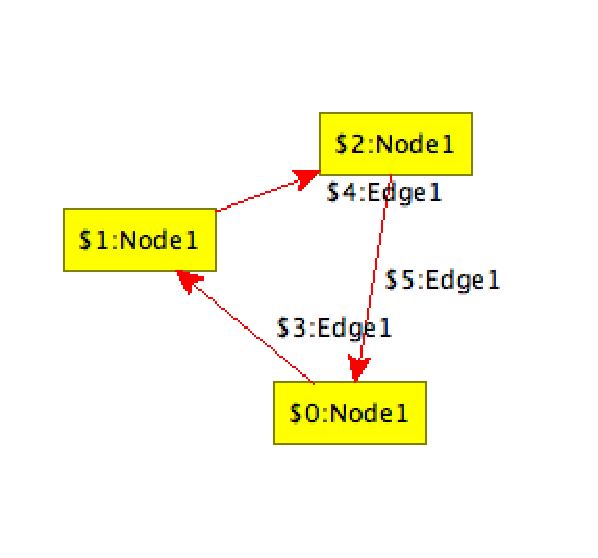
\includegraphics[width=0.3\linewidth]{fig/debug0tra}
\end{center}
We type \texttt{d}(etailed step) to apply \texttt{makeFlake1} step by step resulting in the following graphs:
\begin{center}
  \parbox{0.2\linewidth}{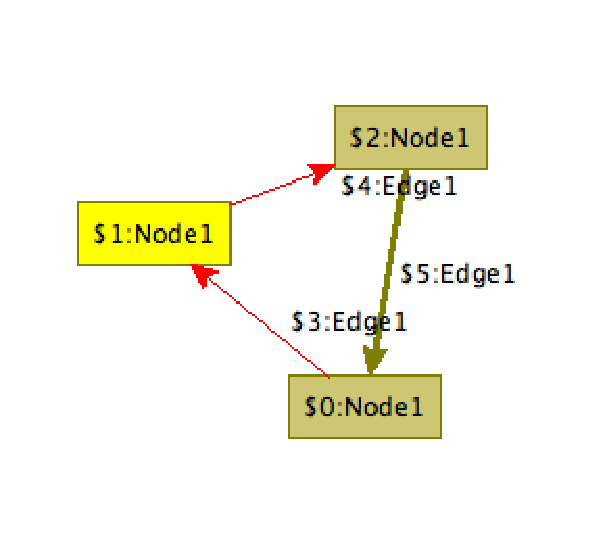
\includegraphics[width=\linewidth]{fig/debug1tra}}\parbox{0.375\linewidth}{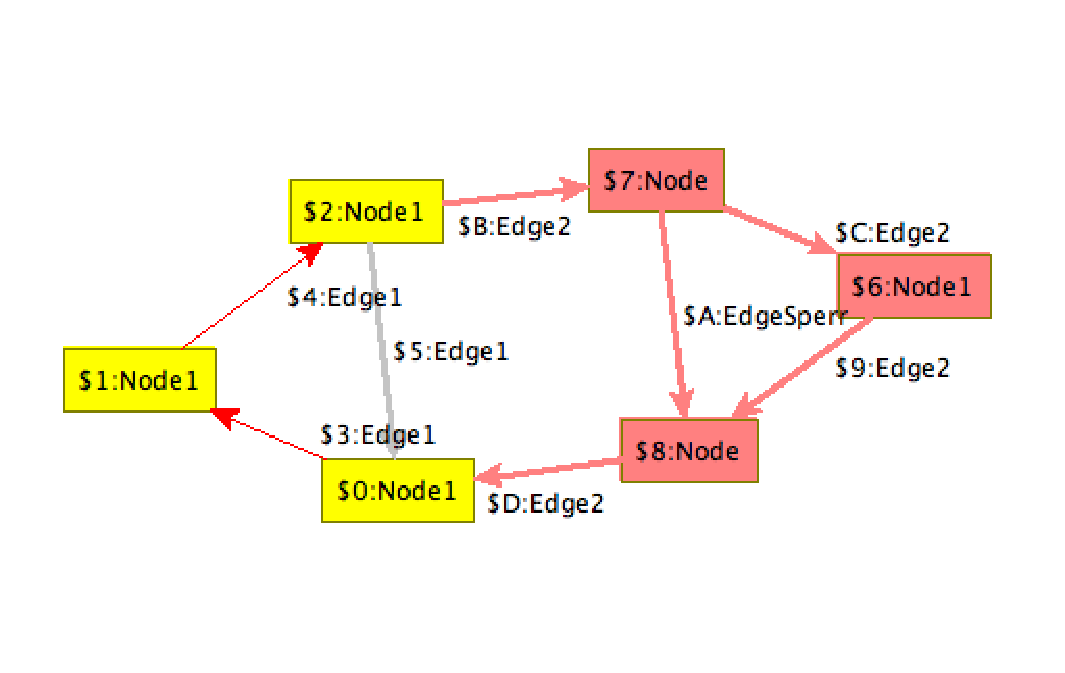
\includegraphics[width=\linewidth]{fig/debug2tra}}\parbox{0.375\linewidth}{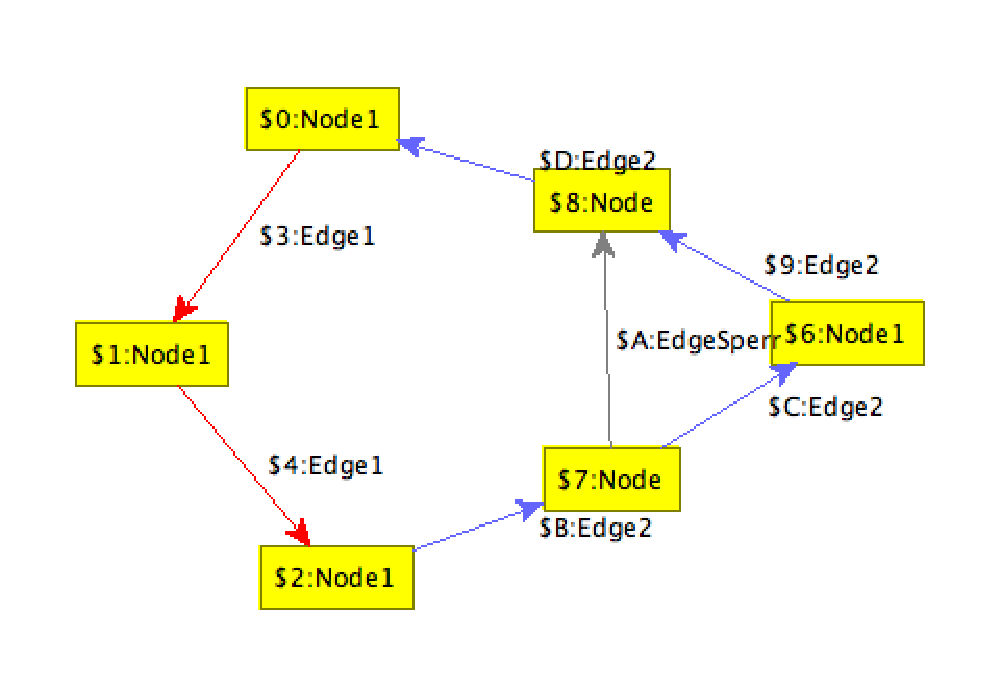
\includegraphics[width=\linewidth]{fig/debug3tra}}
\end{center}
The following table shows the ``break points'' of further debug commands, entered one after another:
\begin{center}
  \begin{tabular}{|l|l|} \hline
    \textbf{Command} & \textbf{Active rule} \\ \hline
    \texttt{s} & \texttt{makeFlake1} \\
    \texttt{o} & \texttt{beautify} \\
    \texttt{s} & \texttt{doNothing} \\
    \texttt{s} & \texttt{beautify} \\ 
    \texttt{n} & \texttt{beautify} \\ 
    \texttt{o} & \texttt{makeFlake2} \\
    \texttt{r} & --- \\ \hline
  \end{tabular}
\end{center}
\end{example}   
\end{figure}


\section{LGSPBackend Custom Commands}
\label{custom}
The \indexed{LGSPBackend} supports the following custom commands:

\subsection{Graph Related Commands}
\begin{rail}
  'custom' 'graph' analyzegraph
\end{rail}\ixkeyw{custom}\ixkeyw{graph}
Analyzes\indexmain{analyzing graph} the current working graph. The analysis data provides vital information for efficient \indexed{search plan}s. Analysis data is available as long as \GrShell\ is running, i.e.\ when the working graph changes, the analysis data is still available but maybe obsolete.

\subsection{Action Related Commands}
\begin{rail}
  'custom' 'actions' gensearchplan (Action+)
\end{rail}\ixkeyw{custom}\ixkeyw{actions}
Creates a search plan for each rewrite rule \emph{Action} using a heuristic method and the analyzes data (if the graph has been analyzed by \texttt{custom graph analyze\_graph}). Otherwise a \indexed{default search plan} is used. For efficiency reasons it is recommended to do analyzing and search plan creation during the rewriting procedure. Therefore the host graph should be in a stage ``similar'' to the final result. Indeed there might be some trial-and-error steps necessary to get an efficient search plan. A search plan is available as long as the current rule set remains loaded. 
Specify multiple rewrite rules instead of using multiple commands for each rule to improve the search plan generation performance.

\begin{rail}
  'custom' 'actions' setmaxmatches Number
\end{rail}\ixkeyw{custom}\ixkeyw{actions}
Sets the maximum amount of possible pattern matches to \emph{Number}. This command affects the expression \texttt{[\emph{Rule}]}. If \emph{Number} is less or equal to zero, the constraint is reset.




\chapter{Examples}
\label{anexample}
\section{Busy Beaver}
We want \GrG\ to work as hard as a busy beaver \cite{kroll, bb}. Our busy beaver is a turing machine, that has got five states, writes 1,471 bars onto the tape and terminates \cite{beaver}. So first of all we design a turing machine as graph model. Besides this example shows that \GrG\ is turing complete. 

\subsection{Graph Model}
Let's start with
\lstset{language=grgenmodel}
\begin{lstlisting}[name=gr]
model TuringMashine;
\end{lstlisting}

The tape will be a chain of \emph{TapePosition} nodes connected by right edges. A cell value is modeled by a reflexive \emph{value} edge, attached to a \emph{TapePosition} node. The leftmost and the rightmost cell (\emph{TapePosition}) does not have an incoming and outgoing edge respectively. Therefore we have the node constraint $[0:1]$.
\lstset{language=grgenmodel}
\begin{lstlisting}[name=gr]
node class TapePosition; 
edge class right
  connect TapePosition[0:1] -> TapePosition[0:1];
  
edge class value
  connect TapePosition[1] -> TapePosition[1];  
edge class zero extends value;
edge class one extends value;
edge class empty extends value;  
\end{lstlisting}
Finally we need states and transitions. The current configuration is modeled with a \emph{RWHead} edge pointing to a \emph{TapePosition} node. \emph{State} nodes are connected with \emph{WriteValue} nodes via \emph{value} edges and from a \emph{WriteValue} node a \emph{move\dots} edge leads to the next state.
\begin{lstlisting}[name=gr]
node class RWHead;

node class WriteValue;
node class WriteZero extends WriteValue;
node class WriteOne extends WriteValue;
node class WriteEmpty extends WriteValue; 

edge class moveLeft;
edge class moveRight;
edge class dontMove;
\end{lstlisting}

\subsection{Rule Set}
Now the rule set: we start with
\lstset{language=grgenactions}
\begin{lstlisting}[name=grg] 
actions Turing using TuringModel;
\end{lstlisting}
We need rewrite rules for the following steps of the turing machine:
\begin{enumerate}
  \item Reading the value of the current tape cell and select a outgoing edge of the current state.
  \item Writing a new value in the current cell, according to the sub type of the \emph{WriteValue} node.
  \item Move the read-write-head along the tape and propagate a new state as current state. 
\end{enumerate}
As you can see a transition of the turing machine is split into two graph rewriting steps: Writing the new value onto the tape and performing the state transition. We need eleven rules, three rules for each step (for ``zero'', ``one'' and ``empty'') and two rules for extending the tape to the left and the the right, respectively.
\begin{lstlisting}[name=grg] 
rule readZeroRule {
	pattern {
		s:State -:RWHead->tp:TapePosition -zv:zero->tp;
		s -zr:zero-> wv:WriteValue;
	}
	replace {
		s -zr-> wv;
		tp -zv-> tp;
		wv -:RWHead->tp;
	}
}      
\end{lstlisting}
We the state and the current cell (\emph{RWHead} edge) and check, if the cell value is zero. Furthermore we check, if the state has a transition for zero. The replacement part deletes the \emph{RWHead} edge between \emph{s} and \emph{tp} and adds it between \emph{wv} and \emph{tp}. Analogous the remaining rules:
\begin{lstlisting}[name=grg] 
rule readOneRule {
	pattern {
		s:State -:RWHead-> tp:TapePosition -ov:one-> tp;
		s -or:one-> wv:WriteValue;
	}
	replace {
		s -or-> wv;
		tp -ov-> tp;
		wv -:RWHead-> tp;
	}
}

rule readEmptyRule {
	pattern {
		s:State -:RWHead-> tp:TapePosition -ev:empty-> tp;
		s -er:empty-> wv:WriteValue;
	}
	replace {
		s -er-> wv;
		tp -ev-> tp;
		wv -:RWHead-> tp;
	}
}

rule writeZeroRule {
	pattern {
		wv:WriteZero -rw:RWHead-> tp:TapePosition -:value-> tp;
	}
	replace {
		wv -rw-> tp -:zero-> tp;
	}	
}

rule writeOneRule {
	pattern {
		wv:WriteOne -rw:RWHead-> tp:TapePosition -:value-> tp;
	}
	replace {
		wv -rw-> tp -:one-> tp;
	}	
}

rule writeEmptyRule {
	pattern {
		wv:WriteEmpty -rw:RWHead-> tp:TapePosition -:value-> tp;
	}
	replace {
		wv -rw-> tp -:empty-> tp;
	}	
}

rule moveLeftRule {
	pattern {
		wv:WriteValue -m:moveLeft-> s:State;
		wv -:RWHead-> tp:TapePosition <-r:right- ltp:TapePosition;
	}
	replace {
		wv -m-> s;
		s -:RWHead-> ltp -r-> tp;
	}
}

rule moveRightRule {
	pattern {
		wv:WriteValue -m:moveRight-> s:State;
		wv -:RWHead-> tp:TapePosition -r:right-> rtp:TapePosition;
	}
	replace {
		wv -m-> s;
		s -:RWHead-> rtp <-r- tp;
	}
}

rule dontMoveRule {
	pattern {
		wv:WriteValue -m:dontMove-> s:State;
		wv -:RWHead-> tp:TapePosition;
	}
	replace {
		tp;
		wv -m-> s;
		s -:RWHead-> tp;
	}
}

rule ensureMoveLeftValidRule {
	pattern {
		wv:WriteValue -m:moveLeft-> s:State;
		wv -rw:RWHead-> tp:TapePosition;
		negative {
			tp <-:right- ltp:TapePosition;
		}
	}
	replace {
		wv -m-> s;
		wv -rw-> tp <-:right- ltp:TapePosition -:empty-> ltp;
	}
}

rule ensureMoveRightValidRule {
	pattern {
		wv:WriteValue -m:moveRight-> s:State;
		wv -rw:RWHead-> tp:TapePosition;
		negative {
			tp -:right-> rtp:TapePosition;
		}
	}
	replace {
		wv -m-> s;
		wv -rw-> tp -:right-> rtp:TapePosition -:empty-> rtp;
	}
}
\end{lstlisting}
Have a look at the negative condition within the \emph{ensureMove\dots} rules. They ensure, that the current cell is in deed at the end of the tape: an edge to a right / left neighbor cell may not exist.

Finally we construct the busy beaver and let it work with GrShell:
\lstset{language=grshell}
\begin{lstlisting}[name=bb] 
select backend "lgspBackend.dll"
new graph "../lib/lgsp-TuringModel.dll" "Busy Beaver"
select actions "../lib/lgsp-TuringActions.dll"

# Initialize tape
new tp:TapePosition($="Startposition")

# States
new sA:State($="A")
new sB:State($="B")
new sC:State($="C")
new sD:State($="D")
new sE:State($="E")
new sH:State($ = "Halt")

new sA -:RWHead-> tp

# Transitions: three lines per state for
#   - updating cell value
#   - moving read-write-head
# respectively

new sA_0: WriteOne
new sA -:empty-> sA_0
new sA_0 -:moveLeft-> sB

new sA_1: WriteOne
new sA -:one ->sA_1
new sA_1 -:moveLeft->sD

new sB_0: WriteOne
new sB -:empty-> sB_0
new sB_0 -:moveRight-> sC

new sB_1: WriteEmpty
new sB -:one-> sB_1
new sB_1 -:moveRight-> sE

new sC_0: WriteEmpty
new sC -:empty ->sC_0
new sC_0 -:moveLeft->sA

new sC_1: WriteEmpty
new sC -:one-> sC_1
new sC_1 -:moveRight-> sB

new sD_0: WriteOne
new sD -:empty ->sD_0
new sD_0 -:moveLeft->sE

new sD_1: WriteOne
new sD -:one-> sD_1
new sD_1 -:moveLeft-> sH

new sE_0: WriteOne
new sE -:empty ->sE_0
new sE_0 -:moveLeft->sC

new sE_1: WriteOne
new sE -:one-> sE_1
new sE_1 -:moveLeft-> sC
}      
\end{lstlisting}

Our busy beaver looks like this:
\begin{center}
  \fbox{\includegraphics[width=\linewidth]{fig/bbstart}}
\end{center}
The graph rewriting sequence is quite straight forward and generic to the turing graph model. Note that for each state the ``\emph{\dots Empty\dots} | \emph{\dots One\dots}'' selection is unambiguous.
\begin{lstlisting}[name=bb]
  grs ((readOneRule | readEmptyRule) ; (writeOneRule | writeEmptyRule) ; (ensureMoveLeftValidRule | ensureMoveRightValidRule) ; (moveLeftRule | moveRightRule)){32}
\end{lstlisting}
We intercept the machine after 32 iterations and look at the result so far:
\begin{center}
  \fbox{\includegraphics[width=\linewidth]{fig/bbmiddle}}
\end{center}
In order to improve the performance we generate better search plans.
\begin{lstlisting}[name=bb]
custom graph analyze_graph
custom actions gen_searchplan readOneRule
custom actions gen_searchplan readEmptyRule
custom actions gen_searchplan writeOneRule
custom actions gen_searchplan writeEmptyRule
custom actions gen_searchplan ensureMoveLeftValidRule
custom actions gen_searchplan ensureMoveRightValidRule
custom actions gen_searchplan moveLeftRule
custom actions gen_searchplan moveRightRule
\end{lstlisting}

Let the beaver run:
\begin{lstlisting}[name=bb]
  grs ((readOneRule | readEmptyRule) ; (writeOneRule | writeEmptyRule) ; (ensureMoveLeftValidRule | ensureMoveRightValidRule) ; (moveLeftRule | moveRightRule))*
\end{lstlisting}

\section{Fractals}
 

\thebibliography{99}
\bibitem{geiss} R. Geiß et al.: \emph{\GrG: A Fast SPO-Based Graph Rewriting Tool} in Graph Transformations, number 4178 in LNCS, pages 383-397, Springer, 2006
\bibitem{kroll} M. Kroll: \emph{Portierung des C-Anteils des Graphersetzungssystems \GrG\ nach C\# mit Erweiterungen}, Studienarbeit, Fakultät für Informatik, Universität Karlsruhe, 2007
\bibitem{hack} S. Hack: \emph{Graphersetzung für Optimierung in der Codeerzeugung} Diplomarbeit, Fakultät für Informatik, Universität Karlsruhe, 2003
\bibitem{grund} D. Grund: \emph{Negative Anwendungsbedingungen für den Graphersetzer \GrG} Studienarbeit, Fakultät für Informatik, Universität Karlsruhe, 2004 
\bibitem{adam} A. Szalkowski: \emph{Negative Anwendungsbedingungen für das suchprogrammbasierte Backend von GrGen} Studienarbeit, Fakultät für Informatik, Universität Karlsruhe, 2005
\bibitem{batz} G. Batz: \emph{Graphersetzung für eine Zwischendarstellung im Übersetzerbau} Diplomarbeit, Fakultät für Informatik, Universität Karlsruhe, 2005
\bibitem{pascal} K. Jensen, N. Wirth: \emph{Pascal User Manual and Report} Springer, $^41991$
\bibitem{bb} A. Dewdney: \emph{A computer trap for the Busy Beaver, the hardest-working machine} Scientific American, 251(2), pages 10-12, 16, 17, August 1984
\bibitem{beaver} H. Marxen, J. Buntrock: \emph{Old list of record TMs.}\\ http://www.drb.insel.de/~heiner/BB/index.html. Version: August 2000

\end{document}
